%*************************************************************************
% A Classic Thesis Style
% An Homage to The Elements of Typographic Style
%
% Copyright (C) 2017 André Miede and Ivo Pletikosić
%
% If you like the style then I would appreciate a postcard. My address
% can be found in the file ClassicThesis.pdf. A collection of the
% postcards I received so far is available online at
% http://postcards.miede.de
%
% License:
% This program is free software; you can redistribute it and/or modify
% it under the terms of the GNU General Public License as published by
% the Free Software Foundation; either version 2 of the License, or
% (at your option) any later version.
%
% This program is distributed in the hope that it will be useful,
% but WITHOUT ANY WARRANTY; without even the implied warranty of
% MERCHANTABILITY or FITNESS FOR A PARTICULAR PURPOSE.  See the
% GNU General Public License for more details.
%
% You should have received a copy of the GNU General Public License
% along with this program; see the file COPYING.  If not, write to
% the Free Software Foundation, Inc., 59 Temple Place - Suite 330,
% Boston, MA 02111-1307, USA.
%
% PLEASE SEE ALSO THE AUTHORS' NOTE REGARDING THIS LICENSE
% IN THE DOCUMENTATION (ClassicThesis.pdf --> Chapter 1 / Chapter01.tex)
%*************************************************************************
\RequirePackage{silence} % :-\
    \WarningFilter{scrreprt}{Usage of package `titlesec'}
    %\WarningFilter{scrreprt}{Activating an ugly workaround}
    \WarningFilter{titlesec}{Non standard sectioning command detected}
\documentclass[ openright,titlepage,numbers=noenddot,headinclude,%twoside, %1headlines,% letterpaper a4paper
                footinclude=true,cleardoublepage=empty,abstractoff, % <--- obsolete, remove (todo)
                BCOR=5mm,paper=a4,fontsize=11pt,%11pt,a4paper,%
                ngerman,american,%lockflag%
                ]{scrreprt}

%*************************************************************************
% Note: Make all your adjustments in here
%*************************************************************************
% ****************************************************************************************************
% hdathesis-config.tex 
% Use it at the beginning of your thesis.tex, or as a LaTeX Preamble 
% in your thesis.{tex,lyx} with % ****************************************************************************************************
% hdathesis-config.tex 
% Use it at the beginning of your thesis.tex, or as a LaTeX Preamble 
% in your thesis.{tex,lyx} with % ****************************************************************************************************
% hdathesis-config.tex 
% Use it at the beginning of your thesis.tex, or as a LaTeX Preamble 
% in your thesis.{tex,lyx} with \input{hdathesis-config}
% ****************************************************************************************************

% ****************************************************************************************************
% 1. Personal data and user ad-hoc commands
% ****************************************************************************************************
\newcommand{\myTitle}{Entwicklung und Performanceanalyse einer dynamischen Facettensuche auf mobilen Endgeräten\xspace}
%\newcommand{\mySubtitle}{An Homage to The Elements of Typographic Style\xspace}
\newcommand{\myDegree}{Bachelor of Science (B.Sc.)\xspace} 
%\newcommand{\myDegree}{Bachelor of Arts (B.A.)\xspace}
%\newcommand{\myDegree}{Master of Science (M.Sc.)\xspace}
%\newcommand{\myDegree}{Master of Arts (M.A.)\xspace}
\newcommand{\myName}{Fabian Kuch\xspace}
\newcommand{\myId}{765570\xspace}
\newcommand{\myProf}{Dr. Kilian Schwarz\xspace}
\newcommand{\myOtherProf}{Björn Frömmer\xspace}
\newcommand{\myFaculty}{Fachbereich Informatik\xspace}
\newcommand{\myUni}{Hochschule Darmstadt\xspace}
\newcommand{\myLocation}{Darmstadt\xspace}
\newcommand{\myTime}{10. Oktober 2023\xspace}
\newcommand{\myVersion}{version 0.0\xspace}

% ****************************************************************************************************
% 2. Is it a master thesis?
% ****************************************************************************************************
%\PassOptionsToPackage{master}{hdahesis} % uncomment if this is a master thesis 

% ****************************************************************************************************
% 3. Does the thesis have a lock flag?
% ****************************************************************************************************
%\PassOptionsToPackage{lockflag}{hdathesis} % uncomment if this thesis has a lock flag 

% ****************************************************************************************************
% 4. Loading some handy packages
% ****************************************************************************************************
% ****************************************************************************************************
% Packages with options that might require adjustments
% ****************************************************************************************************

%\PassOptionsToPackage{ngerman,american}{babel}   % change this to your language(s)
% Spanish languages need extra options in order to work with this template
%\PassOptionsToPackage{spanish,es-lcroman}{babel}
\usepackage{babel}


% ****************************************************************************************************

% ****************************************************************************************************
% 1. Personal data and user ad-hoc commands
% ****************************************************************************************************
\newcommand{\myTitle}{Entwicklung und Performanceanalyse einer dynamischen Facettensuche auf mobilen Endgeräten\xspace}
%\newcommand{\mySubtitle}{An Homage to The Elements of Typographic Style\xspace}
\newcommand{\myDegree}{Bachelor of Science (B.Sc.)\xspace} 
%\newcommand{\myDegree}{Bachelor of Arts (B.A.)\xspace}
%\newcommand{\myDegree}{Master of Science (M.Sc.)\xspace}
%\newcommand{\myDegree}{Master of Arts (M.A.)\xspace}
\newcommand{\myName}{Fabian Kuch\xspace}
\newcommand{\myId}{765570\xspace}
\newcommand{\myProf}{Dr. Kilian Schwarz\xspace}
\newcommand{\myOtherProf}{Björn Frömmer\xspace}
\newcommand{\myFaculty}{Fachbereich Informatik\xspace}
\newcommand{\myUni}{Hochschule Darmstadt\xspace}
\newcommand{\myLocation}{Darmstadt\xspace}
\newcommand{\myTime}{10. Oktober 2023\xspace}
\newcommand{\myVersion}{version 0.0\xspace}

% ****************************************************************************************************
% 2. Is it a master thesis?
% ****************************************************************************************************
%\PassOptionsToPackage{master}{hdahesis} % uncomment if this is a master thesis 

% ****************************************************************************************************
% 3. Does the thesis have a lock flag?
% ****************************************************************************************************
%\PassOptionsToPackage{lockflag}{hdathesis} % uncomment if this thesis has a lock flag 

% ****************************************************************************************************
% 4. Loading some handy packages
% ****************************************************************************************************
% ****************************************************************************************************
% Packages with options that might require adjustments
% ****************************************************************************************************

%\PassOptionsToPackage{ngerman,american}{babel}   % change this to your language(s)
% Spanish languages need extra options in order to work with this template
%\PassOptionsToPackage{spanish,es-lcroman}{babel}
\usepackage{babel}


% ****************************************************************************************************

% ****************************************************************************************************
% 1. Personal data and user ad-hoc commands
% ****************************************************************************************************
\newcommand{\myTitle}{Entwicklung und Performanceanalyse einer dynamischen Facettensuche auf mobilen Endgeräten\xspace}
%\newcommand{\mySubtitle}{An Homage to The Elements of Typographic Style\xspace}
\newcommand{\myDegree}{Bachelor of Science (B.Sc.)\xspace} 
%\newcommand{\myDegree}{Bachelor of Arts (B.A.)\xspace}
%\newcommand{\myDegree}{Master of Science (M.Sc.)\xspace}
%\newcommand{\myDegree}{Master of Arts (M.A.)\xspace}
\newcommand{\myName}{Fabian Kuch\xspace}
\newcommand{\myId}{765570\xspace}
\newcommand{\myProf}{Dr. Kilian Schwarz\xspace}
\newcommand{\myOtherProf}{Björn Frömmer\xspace}
\newcommand{\myFaculty}{Fachbereich Informatik\xspace}
\newcommand{\myUni}{Hochschule Darmstadt\xspace}
\newcommand{\myLocation}{Darmstadt\xspace}
\newcommand{\myTime}{10. Oktober 2023\xspace}
\newcommand{\myVersion}{version 0.0\xspace}

% ****************************************************************************************************
% 2. Is it a master thesis?
% ****************************************************************************************************
%\PassOptionsToPackage{master}{hdahesis} % uncomment if this is a master thesis 

% ****************************************************************************************************
% 3. Does the thesis have a lock flag?
% ****************************************************************************************************
%\PassOptionsToPackage{lockflag}{hdathesis} % uncomment if this thesis has a lock flag 

% ****************************************************************************************************
% 4. Loading some handy packages
% ****************************************************************************************************
% ****************************************************************************************************
% Packages with options that might require adjustments
% ****************************************************************************************************

%\PassOptionsToPackage{ngerman,american}{babel}   % change this to your language(s)
% Spanish languages need extra options in order to work with this template
%\PassOptionsToPackage{spanish,es-lcroman}{babel}
\usepackage{babel}


% ****************************************************************************************************
% classicthesis-config.tex
% formerly known as loadpackages.sty, classicthesis-ldpkg.sty, and classicthesis-preamble.sty
% Use it at the beginning of your ClassicThesis.tex, or as a LaTeX Preamble
% in your ClassicThesis.{tex,lyx} with % ****************************************************************************************************
% classicthesis-config.tex
% formerly known as loadpackages.sty, classicthesis-ldpkg.sty, and classicthesis-preamble.sty
% Use it at the beginning of your ClassicThesis.tex, or as a LaTeX Preamble
% in your ClassicThesis.{tex,lyx} with % ****************************************************************************************************
% classicthesis-config.tex
% formerly known as loadpackages.sty, classicthesis-ldpkg.sty, and classicthesis-preamble.sty
% Use it at the beginning of your ClassicThesis.tex, or as a LaTeX Preamble
% in your ClassicThesis.{tex,lyx} with \input{classicthesis-config}
% ****************************************************************************************************
% If you like the classicthesis, then I would appreciate a postcard.
% My address can be found in the file ClassicThesis.pdf. A collection
% of the postcards I received so far is available online at
% http://postcards.miede.de
% ****************************************************************************************************


% ****************************************************************************************************
% 0. Set the encoding of your files. UTF-8 is the only sensible encoding nowadays. If you can't read
% äöüßáéçèê∂åëæƒÏ€ then change the encoding setting in your editor, not the line below. If your editor
% does not support utf8 use another editor!
% ****************************************************************************************************
\PassOptionsToPackage{utf8}{inputenc}
  \usepackage{inputenc}

% ****************************************************************************************************
% 1. Configure classicthesis for your needs here, e.g., remove "drafting" below
% in order to deactivate the time-stamp on the pages
% (see ClassicThesis.pdf for more information):
% ****************************************************************************************************
\PassOptionsToPackage{
  drafting=false,   % print version information on the bottom of the pages
  tocaligned=false, % the left column of the toc will be aligned (no indentation)
  dottedtoc=true,   % page numbers in ToC flushed right
  parts=true,       % use part division
  eulerchapternumbers=true, % use AMS Euler for chapter font (otherwise Palatino)
  linedheaders=false,       % chaper headers will have line above and beneath
  floatperchapter=true,     % numbering per chapter for all floats (i.e., Figure 1.1)
  listings=true,    % load listings package and setup LoL
  subfig=true,      % setup for preloaded subfig package
  eulermath=false,  % use awesome Euler fonts for mathematical formulae (only with pdfLaTeX)
  beramono=true,    % toggle a nice monospaced font (w/ bold)
  minionpro=false   % setup for minion pro font; use minion pro small caps as well (only with pdfLaTeX)
}{classicthesis}


% ****************************************************************************************************
% 2. Personal data and user ad-hoc commands
% ****************************************************************************************************
%\newcommand{\myTitle}{A Classic Thesis Style\xspace}
%\newcommand{\mySubtitle}{An Homage to The Elements of Typographic Style\xspace}
%\newcommand{\myDegree}{Doktor-Ingenieur (Dr.-Ing.)\xspace}
%\newcommand{\myName}{André Miede\xspace}
%\newcommand{\myProf}{Put name here\xspace}
%\newcommand{\myOtherProf}{Put name here\xspace}
%\newcommand{\mySupervisor}{Put name here\xspace}
%\newcommand{\myFaculty}{Put data here\xspace}
%\newcommand{\myDepartment}{Put data here\xspace}
%\newcommand{\myUni}{Put data here\xspace}
%\newcommand{\myLocation}{Saarbrücken\xspace}
%\newcommand{\myTime}{October 2017\xspace}
%\newcommand{\myVersion}{version 4.4}

% ********************************************************************
% Setup, finetuning, and useful commands
% ********************************************************************
\newcounter{dummy} % necessary for correct hyperlinks (to index, bib, etc.)
\newlength{\abcd} % for ab..z string length calculation
\providecommand{\mLyX}{L\kern-.1667em\lower.25em\hbox{Y}\kern-.125emX\@}
\newcommand{\ie}{i.\,e.}
\newcommand{\Ie}{I.\,e.}
\newcommand{\eg}{e.\,g.}
\newcommand{\Eg}{E.\,g.}
% ****************************************************************************************************


% ****************************************************************************************************
% 3. Loading some handy packages
% ****************************************************************************************************
% ********************************************************************
% Packages with options that might require adjustments
% ********************************************************************
%\PassOptionsToPackage{ngerman,american}{babel}   % change this to your language(s), main language last
% Spanish languages need extra options in order to work with this template
%\PassOptionsToPackage{spanish,es-lcroman}{babel}
\usepackage{babel}

\usepackage{csquotes}

\PassOptionsToPackage{%
  %backend=biber,bibencoding=utf8, %instead of bibtex
  backend=bibtex8,bibencoding=ascii,%
  language=auto,%
  %style=numeric-comp,%
  style=alphabetic,%
  %style=authoryear-comp, % Author 1999, 2010
  %bibstyle=authoryear,dashed=false, % dashed: substitute rep. author with ---
  sorting=nyt, % name, year, title
  maxbibnames=10, % default: 3, et al.
  %backref=true,%
  natbib=true % natbib compatibility mode (\citep and \citet still work)
}{biblatex}
  \usepackage{biblatex}

\PassOptionsToPackage{fleqn}{amsmath}       % math environments and more by the AMS
  \usepackage{amsmath}

\PassOptionsToPackage{doublespacing}{hdathesis}  % options: abbrev exam big wiwi english master
  \usepackage{hdathesis}

% ********************************************************************
% General useful packages
% ********************************************************************
\PassOptionsToPackage{T1}{fontenc} % T2A for cyrillics
  \usepackage{fontenc}
\usepackage{textcomp} % fix warning with missing font shapes
\usepackage{scrhack} % fix warnings when using KOMA with listings package
\usepackage{xspace} % to get the spacing after macros right
\usepackage{mparhack} % get marginpar right
%\usepackage{fixltx2e} % fixes some LaTeX stuff --> since 2015 in the LaTeX kernel (see below)
% \usepackage[latest]{latexrelease} % emulate newer kernel version if older is detected
\PassOptionsToPackage{printonlyused,smaller}{acronym}
  \usepackage{acronym} % nice macros for handling all acronyms in the thesis
  %\renewcommand{\bflabel}[1]{{#1}\hfill} % fix the list of acronyms --> no longer working
  %\renewcommand*{\acsfont}[1]{\textsc{#1}}
  %\renewcommand*{\aclabelfont}[1]{\acsfont{#1}}
  %\def\bflabel#1{{#1\hfill}}
  \def\bflabel#1{{\acsfont{#1}\hfill}}
  \def\aclabelfont#1{\acsfont{#1}}
% ****************************************************************************************************
%\usepackage{pgfplots} % External TikZ/PGF support (thanks to Andreas Nautsch)
%\usetikzlibrary{external}
%\tikzexternalize[mode=list and make, prefix=ext-tikz/]
% ****************************************************************************************************


% ****************************************************************************************************
% 4. Setup floats: tables, (sub)figures, and captions
% ****************************************************************************************************
\usepackage{tabularx} % better tables
  \setlength{\extrarowheight}{3pt} % increase table row height
\newcommand{\tableheadline}[1]{\multicolumn{1}{c}{\spacedlowsmallcaps{#1}}}
\newcommand{\myfloatalign}{\centering} % to be used with each float for alignment
\usepackage{caption}
% Thanks to cgnieder and Claus Lahiri
% http://tex.stackexchange.com/questions/69349/spacedlowsmallcaps-in-caption-label
% [REMOVED DUE TO OTHER PROBLEMS, SEE ISSUE #82]
%\DeclareCaptionLabelFormat{smallcaps}{\bothIfFirst{#1}{~}\MakeTextLowercase{\textsc{#2}}}
%\captionsetup{font=small,labelformat=smallcaps} % format=hang,
\captionsetup{font=small} % format=hang,
\usepackage{subfig}
% ****************************************************************************************************


% ****************************************************************************************************
% 5. Setup code listings
% ****************************************************************************************************
\usepackage{listings}
%\lstset{emph={trueIndex,root},emphstyle=\color{BlueViolet}}%\underbar} % for special keywords
\lstset{language=[LaTeX]Tex,%C++,
  morekeywords={PassOptionsToPackage,selectlanguage},
  keywordstyle=\color{RoyalBlue},%\bfseries,
  basicstyle=\small\ttfamily,
  %identifierstyle=\color{NavyBlue},
  commentstyle=\color{Green}\ttfamily,
  stringstyle=\rmfamily,
  numbers=none,%left,%
  numberstyle=\scriptsize,%\tiny
  stepnumber=5,
  numbersep=8pt,
  showstringspaces=false,
  breaklines=true,
  %frameround=ftff,
  %frame=single,
  belowcaptionskip=.75\baselineskip
  %frame=L
}
% ****************************************************************************************************


% ****************************************************************************************************
% 6. PDFLaTeX, hyperreferences, and citation backreferences
% ****************************************************************************************************
% ********************************************************************
% Using PDFLaTeX
% ********************************************************************
\PassOptionsToPackage{hyperfootnotes=false,pdfpagelabels}{hyperref}
  \usepackage{hyperref}  % backref linktocpage pagebackref
%\ifpdf
%\pdfcompresslevel=9
%\pdfadjustspacing=1
%\fi
%\PassOptionsToPackage{pdftex}{graphicx} %%%IVO: driver will be chosen automatically
  \usepackage{graphicx}


% ********************************************************************
% Hyperreferences
% ********************************************************************
\hypersetup{%
  %draft, % hyperref's draft mode, for printing see below
  colorlinks=true, linktocpage=true, pdfstartpage=3, pdfstartview=FitV,%
  % uncomment the following line if you want to have black links (e.g., for printing)
  %colorlinks=false, linktocpage=false, pdfstartpage=3, pdfstartview=FitV, pdfborder={0 0 0},%
  breaklinks=true, pdfpagemode=UseNone, pageanchor=true, pdfpagemode=UseOutlines,%
  plainpages=false, bookmarksnumbered, bookmarksopen=true, bookmarksopenlevel=1,%
  hypertexnames=true, pdfhighlight=/O,%nesting=true,%frenchlinks,%
  urlcolor=webbrown, linkcolor=RoyalBlue, citecolor=webgreen, %pagecolor=RoyalBlue,%
  %urlcolor=Black, linkcolor=Black, citecolor=Black, %pagecolor=Black,%
  pdftitle={\myTitle},%
  pdfauthor={\textcopyright\ \myName, \myUni, \myFaculty},%
  pdfsubject={},%
  pdfkeywords={},%
  pdfcreator={pdfLaTeX},%
  pdfproducer={LaTeX with hyperref and classicthesis}%
}

% ********************************************************************
% Setup autoreferences
% ********************************************************************
% There are some issues regarding autorefnames
% http://www.ureader.de/msg/136221647.aspx
% http://www.tex.ac.uk/cgi-bin/texfaq2html?label=latexwords
% you have to redefine the makros for the
% language you use, e.g., american, ngerman
% (as chosen when loading babel/AtBeginDocument)
% ********************************************************************
\makeatletter
\@ifpackageloaded{babel}%
  {%
    \addto\extrasamerican{%
      \renewcommand*{\figureautorefname}{Figure}%
      \renewcommand*{\tableautorefname}{Table}%
      \renewcommand*{\partautorefname}{Part}%
      \renewcommand*{\chapterautorefname}{Chapter}%
      \renewcommand*{\sectionautorefname}{Section}%
      \renewcommand*{\subsectionautorefname}{Section}%
      \renewcommand*{\subsubsectionautorefname}{Section}%
    }%
    \addto\extrasngerman{%
      \renewcommand*{\paragraphautorefname}{Absatz}%
      \renewcommand*{\subparagraphautorefname}{Unterabsatz}%
      \renewcommand*{\footnoteautorefname}{Fu\"snote}%
      \renewcommand*{\FancyVerbLineautorefname}{Zeile}%
      \renewcommand*{\theoremautorefname}{Theorem}%
      \renewcommand*{\appendixautorefname}{Anhang}%
      \renewcommand*{\equationautorefname}{Gleichung}%
      \renewcommand*{\itemautorefname}{Punkt}%
    }%
      % Fix to getting autorefs for subfigures right (thanks to Belinda Vogt for changing the definition)
      \providecommand{\subfigureautorefname}{\figureautorefname}%
    }{\relax}
\makeatother


% ****************************************************************************************************
% 7. Last calls before the bar closes
% ****************************************************************************************************
% ********************************************************************
% Development Stuff
% ********************************************************************
\listfiles
%\PassOptionsToPackage{l2tabu,orthodox,abort}{nag}
%  \usepackage{nag}
%\PassOptionsToPackage{warning, all}{onlyamsmath}
%  \usepackage{onlyamsmath}

% ********************************************************************
% Last, but not least...
% ********************************************************************
\usepackage{classicthesis}
% ****************************************************************************************************


% ****************************************************************************************************
% 8. Further adjustments (experimental)
% ****************************************************************************************************
% ********************************************************************
% Changing the text area
% ********************************************************************
%\areaset[current]{312pt}{761pt} % 686 (factor 2.2) + 33 head + 42 head \the\footskip
%\setlength{\marginparwidth}{7em}%
%\setlength{\marginparsep}{2em}%

% ********************************************************************
% Using different fonts
% ********************************************************************
%\usepackage[oldstylenums]{kpfonts} % oldstyle notextcomp
%\usepackage[osf]{libertine}
%\usepackage[light,condensed,math]{iwona}
%\renewcommand{\sfdefault}{iwona}
%\usepackage{lmodern} % <-- no osf support :-(
%\usepackage{cfr-lm} %
%\usepackage[urw-garamond]{mathdesign} <-- no osf support :-(
%\usepackage[default,osfigures]{opensans} % scale=0.95
%\usepackage[sfdefault]{FiraSans}
% ********************************************************************
% \usepackage[largesc,osf]{newpxtext}
% Used to fix these:
% https://bitbucket.org/amiede/classicthesis/issues/139/italics-in-pallatino-capitals-chapter
% https://bitbucket.org/amiede/classicthesis/issues/45/problema-testatine-su-classicthesis-style
% ********************************************************************
%\linespread{1.05} % a bit more for Palatino
% ****************************************************************************************************

% ****************************************************************************************************
% If you like the classicthesis, then I would appreciate a postcard.
% My address can be found in the file ClassicThesis.pdf. A collection
% of the postcards I received so far is available online at
% http://postcards.miede.de
% ****************************************************************************************************


% ****************************************************************************************************
% 0. Set the encoding of your files. UTF-8 is the only sensible encoding nowadays. If you can't read
% äöüßáéçèê∂åëæƒÏ€ then change the encoding setting in your editor, not the line below. If your editor
% does not support utf8 use another editor!
% ****************************************************************************************************
\PassOptionsToPackage{utf8}{inputenc}
  \usepackage{inputenc}

% ****************************************************************************************************
% 1. Configure classicthesis for your needs here, e.g., remove "drafting" below
% in order to deactivate the time-stamp on the pages
% (see ClassicThesis.pdf for more information):
% ****************************************************************************************************
\PassOptionsToPackage{
  drafting=false,   % print version information on the bottom of the pages
  tocaligned=false, % the left column of the toc will be aligned (no indentation)
  dottedtoc=true,   % page numbers in ToC flushed right
  parts=true,       % use part division
  eulerchapternumbers=true, % use AMS Euler for chapter font (otherwise Palatino)
  linedheaders=false,       % chaper headers will have line above and beneath
  floatperchapter=true,     % numbering per chapter for all floats (i.e., Figure 1.1)
  listings=true,    % load listings package and setup LoL
  subfig=true,      % setup for preloaded subfig package
  eulermath=false,  % use awesome Euler fonts for mathematical formulae (only with pdfLaTeX)
  beramono=true,    % toggle a nice monospaced font (w/ bold)
  minionpro=false   % setup for minion pro font; use minion pro small caps as well (only with pdfLaTeX)
}{classicthesis}


% ****************************************************************************************************
% 2. Personal data and user ad-hoc commands
% ****************************************************************************************************
%\newcommand{\myTitle}{A Classic Thesis Style\xspace}
%\newcommand{\mySubtitle}{An Homage to The Elements of Typographic Style\xspace}
%\newcommand{\myDegree}{Doktor-Ingenieur (Dr.-Ing.)\xspace}
%\newcommand{\myName}{André Miede\xspace}
%\newcommand{\myProf}{Put name here\xspace}
%\newcommand{\myOtherProf}{Put name here\xspace}
%\newcommand{\mySupervisor}{Put name here\xspace}
%\newcommand{\myFaculty}{Put data here\xspace}
%\newcommand{\myDepartment}{Put data here\xspace}
%\newcommand{\myUni}{Put data here\xspace}
%\newcommand{\myLocation}{Saarbrücken\xspace}
%\newcommand{\myTime}{October 2017\xspace}
%\newcommand{\myVersion}{version 4.4}

% ********************************************************************
% Setup, finetuning, and useful commands
% ********************************************************************
\newcounter{dummy} % necessary for correct hyperlinks (to index, bib, etc.)
\newlength{\abcd} % for ab..z string length calculation
\providecommand{\mLyX}{L\kern-.1667em\lower.25em\hbox{Y}\kern-.125emX\@}
\newcommand{\ie}{i.\,e.}
\newcommand{\Ie}{I.\,e.}
\newcommand{\eg}{e.\,g.}
\newcommand{\Eg}{E.\,g.}
% ****************************************************************************************************


% ****************************************************************************************************
% 3. Loading some handy packages
% ****************************************************************************************************
% ********************************************************************
% Packages with options that might require adjustments
% ********************************************************************
%\PassOptionsToPackage{ngerman,american}{babel}   % change this to your language(s), main language last
% Spanish languages need extra options in order to work with this template
%\PassOptionsToPackage{spanish,es-lcroman}{babel}
\usepackage{babel}

\usepackage{csquotes}

\PassOptionsToPackage{%
  %backend=biber,bibencoding=utf8, %instead of bibtex
  backend=bibtex8,bibencoding=ascii,%
  language=auto,%
  %style=numeric-comp,%
  style=alphabetic,%
  %style=authoryear-comp, % Author 1999, 2010
  %bibstyle=authoryear,dashed=false, % dashed: substitute rep. author with ---
  sorting=nyt, % name, year, title
  maxbibnames=10, % default: 3, et al.
  %backref=true,%
  natbib=true % natbib compatibility mode (\citep and \citet still work)
}{biblatex}
  \usepackage{biblatex}

\PassOptionsToPackage{fleqn}{amsmath}       % math environments and more by the AMS
  \usepackage{amsmath}

\PassOptionsToPackage{doublespacing}{hdathesis}  % options: abbrev exam big wiwi english master
  \usepackage{hdathesis}

% ********************************************************************
% General useful packages
% ********************************************************************
\PassOptionsToPackage{T1}{fontenc} % T2A for cyrillics
  \usepackage{fontenc}
\usepackage{textcomp} % fix warning with missing font shapes
\usepackage{scrhack} % fix warnings when using KOMA with listings package
\usepackage{xspace} % to get the spacing after macros right
\usepackage{mparhack} % get marginpar right
%\usepackage{fixltx2e} % fixes some LaTeX stuff --> since 2015 in the LaTeX kernel (see below)
% \usepackage[latest]{latexrelease} % emulate newer kernel version if older is detected
\PassOptionsToPackage{printonlyused,smaller}{acronym}
  \usepackage{acronym} % nice macros for handling all acronyms in the thesis
  %\renewcommand{\bflabel}[1]{{#1}\hfill} % fix the list of acronyms --> no longer working
  %\renewcommand*{\acsfont}[1]{\textsc{#1}}
  %\renewcommand*{\aclabelfont}[1]{\acsfont{#1}}
  %\def\bflabel#1{{#1\hfill}}
  \def\bflabel#1{{\acsfont{#1}\hfill}}
  \def\aclabelfont#1{\acsfont{#1}}
% ****************************************************************************************************
%\usepackage{pgfplots} % External TikZ/PGF support (thanks to Andreas Nautsch)
%\usetikzlibrary{external}
%\tikzexternalize[mode=list and make, prefix=ext-tikz/]
% ****************************************************************************************************


% ****************************************************************************************************
% 4. Setup floats: tables, (sub)figures, and captions
% ****************************************************************************************************
\usepackage{tabularx} % better tables
  \setlength{\extrarowheight}{3pt} % increase table row height
\newcommand{\tableheadline}[1]{\multicolumn{1}{c}{\spacedlowsmallcaps{#1}}}
\newcommand{\myfloatalign}{\centering} % to be used with each float for alignment
\usepackage{caption}
% Thanks to cgnieder and Claus Lahiri
% http://tex.stackexchange.com/questions/69349/spacedlowsmallcaps-in-caption-label
% [REMOVED DUE TO OTHER PROBLEMS, SEE ISSUE #82]
%\DeclareCaptionLabelFormat{smallcaps}{\bothIfFirst{#1}{~}\MakeTextLowercase{\textsc{#2}}}
%\captionsetup{font=small,labelformat=smallcaps} % format=hang,
\captionsetup{font=small} % format=hang,
\usepackage{subfig}
% ****************************************************************************************************


% ****************************************************************************************************
% 5. Setup code listings
% ****************************************************************************************************
\usepackage{listings}
%\lstset{emph={trueIndex,root},emphstyle=\color{BlueViolet}}%\underbar} % for special keywords
\lstset{language=[LaTeX]Tex,%C++,
  morekeywords={PassOptionsToPackage,selectlanguage},
  keywordstyle=\color{RoyalBlue},%\bfseries,
  basicstyle=\small\ttfamily,
  %identifierstyle=\color{NavyBlue},
  commentstyle=\color{Green}\ttfamily,
  stringstyle=\rmfamily,
  numbers=none,%left,%
  numberstyle=\scriptsize,%\tiny
  stepnumber=5,
  numbersep=8pt,
  showstringspaces=false,
  breaklines=true,
  %frameround=ftff,
  %frame=single,
  belowcaptionskip=.75\baselineskip
  %frame=L
}
% ****************************************************************************************************


% ****************************************************************************************************
% 6. PDFLaTeX, hyperreferences, and citation backreferences
% ****************************************************************************************************
% ********************************************************************
% Using PDFLaTeX
% ********************************************************************
\PassOptionsToPackage{hyperfootnotes=false,pdfpagelabels}{hyperref}
  \usepackage{hyperref}  % backref linktocpage pagebackref
%\ifpdf
%\pdfcompresslevel=9
%\pdfadjustspacing=1
%\fi
%\PassOptionsToPackage{pdftex}{graphicx} %%%IVO: driver will be chosen automatically
  \usepackage{graphicx}


% ********************************************************************
% Hyperreferences
% ********************************************************************
\hypersetup{%
  %draft, % hyperref's draft mode, for printing see below
  colorlinks=true, linktocpage=true, pdfstartpage=3, pdfstartview=FitV,%
  % uncomment the following line if you want to have black links (e.g., for printing)
  %colorlinks=false, linktocpage=false, pdfstartpage=3, pdfstartview=FitV, pdfborder={0 0 0},%
  breaklinks=true, pdfpagemode=UseNone, pageanchor=true, pdfpagemode=UseOutlines,%
  plainpages=false, bookmarksnumbered, bookmarksopen=true, bookmarksopenlevel=1,%
  hypertexnames=true, pdfhighlight=/O,%nesting=true,%frenchlinks,%
  urlcolor=webbrown, linkcolor=RoyalBlue, citecolor=webgreen, %pagecolor=RoyalBlue,%
  %urlcolor=Black, linkcolor=Black, citecolor=Black, %pagecolor=Black,%
  pdftitle={\myTitle},%
  pdfauthor={\textcopyright\ \myName, \myUni, \myFaculty},%
  pdfsubject={},%
  pdfkeywords={},%
  pdfcreator={pdfLaTeX},%
  pdfproducer={LaTeX with hyperref and classicthesis}%
}

% ********************************************************************
% Setup autoreferences
% ********************************************************************
% There are some issues regarding autorefnames
% http://www.ureader.de/msg/136221647.aspx
% http://www.tex.ac.uk/cgi-bin/texfaq2html?label=latexwords
% you have to redefine the makros for the
% language you use, e.g., american, ngerman
% (as chosen when loading babel/AtBeginDocument)
% ********************************************************************
\makeatletter
\@ifpackageloaded{babel}%
  {%
    \addto\extrasamerican{%
      \renewcommand*{\figureautorefname}{Figure}%
      \renewcommand*{\tableautorefname}{Table}%
      \renewcommand*{\partautorefname}{Part}%
      \renewcommand*{\chapterautorefname}{Chapter}%
      \renewcommand*{\sectionautorefname}{Section}%
      \renewcommand*{\subsectionautorefname}{Section}%
      \renewcommand*{\subsubsectionautorefname}{Section}%
    }%
    \addto\extrasngerman{%
      \renewcommand*{\paragraphautorefname}{Absatz}%
      \renewcommand*{\subparagraphautorefname}{Unterabsatz}%
      \renewcommand*{\footnoteautorefname}{Fu\"snote}%
      \renewcommand*{\FancyVerbLineautorefname}{Zeile}%
      \renewcommand*{\theoremautorefname}{Theorem}%
      \renewcommand*{\appendixautorefname}{Anhang}%
      \renewcommand*{\equationautorefname}{Gleichung}%
      \renewcommand*{\itemautorefname}{Punkt}%
    }%
      % Fix to getting autorefs for subfigures right (thanks to Belinda Vogt for changing the definition)
      \providecommand{\subfigureautorefname}{\figureautorefname}%
    }{\relax}
\makeatother


% ****************************************************************************************************
% 7. Last calls before the bar closes
% ****************************************************************************************************
% ********************************************************************
% Development Stuff
% ********************************************************************
\listfiles
%\PassOptionsToPackage{l2tabu,orthodox,abort}{nag}
%  \usepackage{nag}
%\PassOptionsToPackage{warning, all}{onlyamsmath}
%  \usepackage{onlyamsmath}

% ********************************************************************
% Last, but not least...
% ********************************************************************
\usepackage{classicthesis}
% ****************************************************************************************************


% ****************************************************************************************************
% 8. Further adjustments (experimental)
% ****************************************************************************************************
% ********************************************************************
% Changing the text area
% ********************************************************************
%\areaset[current]{312pt}{761pt} % 686 (factor 2.2) + 33 head + 42 head \the\footskip
%\setlength{\marginparwidth}{7em}%
%\setlength{\marginparsep}{2em}%

% ********************************************************************
% Using different fonts
% ********************************************************************
%\usepackage[oldstylenums]{kpfonts} % oldstyle notextcomp
%\usepackage[osf]{libertine}
%\usepackage[light,condensed,math]{iwona}
%\renewcommand{\sfdefault}{iwona}
%\usepackage{lmodern} % <-- no osf support :-(
%\usepackage{cfr-lm} %
%\usepackage[urw-garamond]{mathdesign} <-- no osf support :-(
%\usepackage[default,osfigures]{opensans} % scale=0.95
%\usepackage[sfdefault]{FiraSans}
% ********************************************************************
% \usepackage[largesc,osf]{newpxtext}
% Used to fix these:
% https://bitbucket.org/amiede/classicthesis/issues/139/italics-in-pallatino-capitals-chapter
% https://bitbucket.org/amiede/classicthesis/issues/45/problema-testatine-su-classicthesis-style
% ********************************************************************
%\linespread{1.05} % a bit more for Palatino
% ****************************************************************************************************

% ****************************************************************************************************
% If you like the classicthesis, then I would appreciate a postcard.
% My address can be found in the file ClassicThesis.pdf. A collection
% of the postcards I received so far is available online at
% http://postcards.miede.de
% ****************************************************************************************************


% ****************************************************************************************************
% 0. Set the encoding of your files. UTF-8 is the only sensible encoding nowadays. If you can't read
% äöüßáéçèê∂åëæƒÏ€ then change the encoding setting in your editor, not the line below. If your editor
% does not support utf8 use another editor!
% ****************************************************************************************************
\PassOptionsToPackage{utf8}{inputenc}
  \usepackage{inputenc}

% ****************************************************************************************************
% 1. Configure classicthesis for your needs here, e.g., remove "drafting" below
% in order to deactivate the time-stamp on the pages
% (see ClassicThesis.pdf for more information):
% ****************************************************************************************************
\PassOptionsToPackage{
  drafting=false,   % print version information on the bottom of the pages
  tocaligned=false, % the left column of the toc will be aligned (no indentation)
  dottedtoc=true,   % page numbers in ToC flushed right
  parts=true,       % use part division
  eulerchapternumbers=true, % use AMS Euler for chapter font (otherwise Palatino)
  linedheaders=false,       % chaper headers will have line above and beneath
  floatperchapter=true,     % numbering per chapter for all floats (i.e., Figure 1.1)
  listings=true,    % load listings package and setup LoL
  subfig=true,      % setup for preloaded subfig package
  eulermath=false,  % use awesome Euler fonts for mathematical formulae (only with pdfLaTeX)
  beramono=true,    % toggle a nice monospaced font (w/ bold)
  minionpro=false   % setup for minion pro font; use minion pro small caps as well (only with pdfLaTeX)
}{classicthesis}


% ****************************************************************************************************
% 2. Personal data and user ad-hoc commands
% ****************************************************************************************************
%\newcommand{\myTitle}{A Classic Thesis Style\xspace}
%\newcommand{\mySubtitle}{An Homage to The Elements of Typographic Style\xspace}
%\newcommand{\myDegree}{Doktor-Ingenieur (Dr.-Ing.)\xspace}
%\newcommand{\myName}{André Miede\xspace}
%\newcommand{\myProf}{Put name here\xspace}
%\newcommand{\myOtherProf}{Put name here\xspace}
%\newcommand{\mySupervisor}{Put name here\xspace}
%\newcommand{\myFaculty}{Put data here\xspace}
%\newcommand{\myDepartment}{Put data here\xspace}
%\newcommand{\myUni}{Put data here\xspace}
%\newcommand{\myLocation}{Saarbrücken\xspace}
%\newcommand{\myTime}{October 2017\xspace}
%\newcommand{\myVersion}{version 4.4}

% ********************************************************************
% Setup, finetuning, and useful commands
% ********************************************************************
\newcounter{dummy} % necessary for correct hyperlinks (to index, bib, etc.)
\newlength{\abcd} % for ab..z string length calculation
\providecommand{\mLyX}{L\kern-.1667em\lower.25em\hbox{Y}\kern-.125emX\@}
\newcommand{\ie}{i.\,e.}
\newcommand{\Ie}{I.\,e.}
\newcommand{\eg}{e.\,g.}
\newcommand{\Eg}{E.\,g.}
% ****************************************************************************************************


% ****************************************************************************************************
% 3. Loading some handy packages
% ****************************************************************************************************
% ********************************************************************
% Packages with options that might require adjustments
% ********************************************************************
%\PassOptionsToPackage{ngerman,american}{babel}   % change this to your language(s), main language last
% Spanish languages need extra options in order to work with this template
%\PassOptionsToPackage{spanish,es-lcroman}{babel}
\usepackage{babel}

\usepackage{csquotes}

\PassOptionsToPackage{%
  %backend=biber,bibencoding=utf8, %instead of bibtex
  backend=bibtex8,bibencoding=ascii,%
  language=auto,%
  %style=numeric-comp,%
  style=alphabetic,%
  %style=authoryear-comp, % Author 1999, 2010
  %bibstyle=authoryear,dashed=false, % dashed: substitute rep. author with ---
  sorting=nyt, % name, year, title
  maxbibnames=10, % default: 3, et al.
  %backref=true,%
  natbib=true % natbib compatibility mode (\citep and \citet still work)
}{biblatex}
  \usepackage{biblatex}

\PassOptionsToPackage{fleqn}{amsmath}       % math environments and more by the AMS
  \usepackage{amsmath}

\PassOptionsToPackage{doublespacing}{hdathesis}  % options: abbrev exam big wiwi english master
  \usepackage{hdathesis}

% ********************************************************************
% General useful packages
% ********************************************************************
\PassOptionsToPackage{T1}{fontenc} % T2A for cyrillics
  \usepackage{fontenc}
\usepackage{textcomp} % fix warning with missing font shapes
\usepackage{scrhack} % fix warnings when using KOMA with listings package
\usepackage{xspace} % to get the spacing after macros right
\usepackage{mparhack} % get marginpar right
%\usepackage{fixltx2e} % fixes some LaTeX stuff --> since 2015 in the LaTeX kernel (see below)
% \usepackage[latest]{latexrelease} % emulate newer kernel version if older is detected
\PassOptionsToPackage{printonlyused,smaller}{acronym}
  \usepackage{acronym} % nice macros for handling all acronyms in the thesis
  %\renewcommand{\bflabel}[1]{{#1}\hfill} % fix the list of acronyms --> no longer working
  %\renewcommand*{\acsfont}[1]{\textsc{#1}}
  %\renewcommand*{\aclabelfont}[1]{\acsfont{#1}}
  %\def\bflabel#1{{#1\hfill}}
  \def\bflabel#1{{\acsfont{#1}\hfill}}
  \def\aclabelfont#1{\acsfont{#1}}
% ****************************************************************************************************
%\usepackage{pgfplots} % External TikZ/PGF support (thanks to Andreas Nautsch)
%\usetikzlibrary{external}
%\tikzexternalize[mode=list and make, prefix=ext-tikz/]
% ****************************************************************************************************


% ****************************************************************************************************
% 4. Setup floats: tables, (sub)figures, and captions
% ****************************************************************************************************
\usepackage{tabularx} % better tables
  \setlength{\extrarowheight}{3pt} % increase table row height
\newcommand{\tableheadline}[1]{\multicolumn{1}{c}{\spacedlowsmallcaps{#1}}}
\newcommand{\myfloatalign}{\centering} % to be used with each float for alignment
\usepackage{caption}
% Thanks to cgnieder and Claus Lahiri
% http://tex.stackexchange.com/questions/69349/spacedlowsmallcaps-in-caption-label
% [REMOVED DUE TO OTHER PROBLEMS, SEE ISSUE #82]
%\DeclareCaptionLabelFormat{smallcaps}{\bothIfFirst{#1}{~}\MakeTextLowercase{\textsc{#2}}}
%\captionsetup{font=small,labelformat=smallcaps} % format=hang,
\captionsetup{font=small} % format=hang,
\usepackage{subfig}
% ****************************************************************************************************


% ****************************************************************************************************
% 5. Setup code listings
% ****************************************************************************************************
\usepackage{listings}
%\lstset{emph={trueIndex,root},emphstyle=\color{BlueViolet}}%\underbar} % for special keywords
\lstset{language=[LaTeX]Tex,%C++,
  morekeywords={PassOptionsToPackage,selectlanguage},
  keywordstyle=\color{RoyalBlue},%\bfseries,
  basicstyle=\small\ttfamily,
  %identifierstyle=\color{NavyBlue},
  commentstyle=\color{Green}\ttfamily,
  stringstyle=\rmfamily,
  numbers=none,%left,%
  numberstyle=\scriptsize,%\tiny
  stepnumber=5,
  numbersep=8pt,
  showstringspaces=false,
  breaklines=true,
  %frameround=ftff,
  %frame=single,
  belowcaptionskip=.75\baselineskip
  %frame=L
}
% ****************************************************************************************************


% ****************************************************************************************************
% 6. PDFLaTeX, hyperreferences, and citation backreferences
% ****************************************************************************************************
% ********************************************************************
% Using PDFLaTeX
% ********************************************************************
\PassOptionsToPackage{hyperfootnotes=false,pdfpagelabels}{hyperref}
  \usepackage{hyperref}  % backref linktocpage pagebackref
%\ifpdf
%\pdfcompresslevel=9
%\pdfadjustspacing=1
%\fi
%\PassOptionsToPackage{pdftex}{graphicx} %%%IVO: driver will be chosen automatically
  \usepackage{graphicx}


% ********************************************************************
% Hyperreferences
% ********************************************************************
\hypersetup{%
  %draft, % hyperref's draft mode, for printing see below
  colorlinks=true, linktocpage=true, pdfstartpage=3, pdfstartview=FitV,%
  % uncomment the following line if you want to have black links (e.g., for printing)
  %colorlinks=false, linktocpage=false, pdfstartpage=3, pdfstartview=FitV, pdfborder={0 0 0},%
  breaklinks=true, pdfpagemode=UseNone, pageanchor=true, pdfpagemode=UseOutlines,%
  plainpages=false, bookmarksnumbered, bookmarksopen=true, bookmarksopenlevel=1,%
  hypertexnames=true, pdfhighlight=/O,%nesting=true,%frenchlinks,%
  urlcolor=webbrown, linkcolor=RoyalBlue, citecolor=webgreen, %pagecolor=RoyalBlue,%
  %urlcolor=Black, linkcolor=Black, citecolor=Black, %pagecolor=Black,%
  pdftitle={\myTitle},%
  pdfauthor={\textcopyright\ \myName, \myUni, \myFaculty},%
  pdfsubject={},%
  pdfkeywords={},%
  pdfcreator={pdfLaTeX},%
  pdfproducer={LaTeX with hyperref and classicthesis}%
}

% ********************************************************************
% Setup autoreferences
% ********************************************************************
% There are some issues regarding autorefnames
% http://www.ureader.de/msg/136221647.aspx
% http://www.tex.ac.uk/cgi-bin/texfaq2html?label=latexwords
% you have to redefine the makros for the
% language you use, e.g., american, ngerman
% (as chosen when loading babel/AtBeginDocument)
% ********************************************************************
\makeatletter
\@ifpackageloaded{babel}%
  {%
    \addto\extrasamerican{%
      \renewcommand*{\figureautorefname}{Figure}%
      \renewcommand*{\tableautorefname}{Table}%
      \renewcommand*{\partautorefname}{Part}%
      \renewcommand*{\chapterautorefname}{Chapter}%
      \renewcommand*{\sectionautorefname}{Section}%
      \renewcommand*{\subsectionautorefname}{Section}%
      \renewcommand*{\subsubsectionautorefname}{Section}%
    }%
    \addto\extrasngerman{%
      \renewcommand*{\paragraphautorefname}{Absatz}%
      \renewcommand*{\subparagraphautorefname}{Unterabsatz}%
      \renewcommand*{\footnoteautorefname}{Fu\"snote}%
      \renewcommand*{\FancyVerbLineautorefname}{Zeile}%
      \renewcommand*{\theoremautorefname}{Theorem}%
      \renewcommand*{\appendixautorefname}{Anhang}%
      \renewcommand*{\equationautorefname}{Gleichung}%
      \renewcommand*{\itemautorefname}{Punkt}%
    }%
      % Fix to getting autorefs for subfigures right (thanks to Belinda Vogt for changing the definition)
      \providecommand{\subfigureautorefname}{\figureautorefname}%
    }{\relax}
\makeatother


% ****************************************************************************************************
% 7. Last calls before the bar closes
% ****************************************************************************************************
% ********************************************************************
% Development Stuff
% ********************************************************************
\listfiles
%\PassOptionsToPackage{l2tabu,orthodox,abort}{nag}
%  \usepackage{nag}
%\PassOptionsToPackage{warning, all}{onlyamsmath}
%  \usepackage{onlyamsmath}

% ********************************************************************
% Last, but not least...
% ********************************************************************
\usepackage{classicthesis}
% ****************************************************************************************************


% ****************************************************************************************************
% 8. Further adjustments (experimental)
% ****************************************************************************************************
% ********************************************************************
% Changing the text area
% ********************************************************************
%\areaset[current]{312pt}{761pt} % 686 (factor 2.2) + 33 head + 42 head \the\footskip
%\setlength{\marginparwidth}{7em}%
%\setlength{\marginparsep}{2em}%

% ********************************************************************
% Using different fonts
% ********************************************************************
%\usepackage[oldstylenums]{kpfonts} % oldstyle notextcomp
%\usepackage[osf]{libertine}
%\usepackage[light,condensed,math]{iwona}
%\renewcommand{\sfdefault}{iwona}
%\usepackage{lmodern} % <-- no osf support :-(
%\usepackage{cfr-lm} %
%\usepackage[urw-garamond]{mathdesign} <-- no osf support :-(
%\usepackage[default,osfigures]{opensans} % scale=0.95
%\usepackage[sfdefault]{FiraSans}
% ********************************************************************
% \usepackage[largesc,osf]{newpxtext}
% Used to fix these:
% https://bitbucket.org/amiede/classicthesis/issues/139/italics-in-pallatino-capitals-chapter
% https://bitbucket.org/amiede/classicthesis/issues/45/problema-testatine-su-classicthesis-style
% ********************************************************************
%\linespread{1.05} % a bit more for Palatino
% ****************************************************************************************************


%*************************************************************************
% Bibliographies
%*************************************************************************
\addbibresource{bibliography.bib}

%*************************************************************************
% Hyphenation
%*************************************************************************
%\hyphenation{put special hyphenation here}

%*************************************************************************
% GO!GO!GO! MOVE IT!
%*************************************************************************
\begin{document}
\frenchspacing
\raggedbottom
\selectlanguage{ngerman} % ngerman, american
%\renewcommand*{\bibname}{new name}
%\setbibpreamble{}
\pagenumbering{roman}
\pagestyle{plain}
%*************************************************************************
% Frontmatter
%*************************************************************************
%*******************************************************
% Titlepage
%*******************************************************
%%%
%%% title page (german)
%%%
\thispagestyle{empty}
\pdfbookmark[0]{Titelblatt}{title}
\begin{titlepage}

  % If printed on two sides, center the title page
  \condTWOSIDE{\changetext{}{19mm}{}{19mm}{}}

  \vspace{1cm}
  \begin{center}
    
\includegraphics[width=7.7cm]{gfx/logo_h-da_rot} \\ 
  \end{center}

  \begin{center}
    \vspace{0.1cm}
    \huge \textbf{\myUni}\\
    \vspace{0.4cm}
    \LARGE --~\myFaculty~--
  \end{center}

  \vfill
  \vfill

  \begin{center}
    \LARGE \textbf{\myTitle}
  \end{center} 

  \vfill
  \vfill

  \begin{center}
    \Large Abschlussarbeit zur Erlangung des akademischen Grades\\
    \vspace{0.3cm}
    \Large \myDegree
  \end{center}

  \vfill

  \begin{center}
    \Large vorgelegt von\\
    \vspace{0.3cm}
    \Large \textbf{\myName}\\
    \vspace{0.3cm}
    \normalsize Matrikelnummer: \myId
  \end{center}

  \vfill
  \vfill

  \begin{center}
    \begin{tabular}{lll}
      Referent    & : & \myProf \\
      Korreferent & : & \myOtherProf
    \end{tabular}
  \end{center} 

  % If printed on two sides, center the title page
  \condTWOSIDE{\changetext{}{-19mm}{}{-19mm}{}}

\end{titlepage}

\thispagestyle{empty}

\hfill

\vfill

\noindent\myName: \textit{\myTitle}, \ifdef{\mySubtitle}{\mySubtitle,}{} %\myDegree,
\textcopyright\ \myTime

%\bigskip
%
%\noindent\spacedlowsmallcaps{Supervisors}: \\
%\myProf \\
%\myOtherProf \\
%\mySupervisor
%
%\medskip
%
%\noindent\spacedlowsmallcaps{Location}: \\
%\myLocation
%
%\medskip
%
%\noindent\spacedlowsmallcaps{Time Frame}: \\
%\myTime

%\cleardoublepage\include{frontbackmatter/Dedication}
%\cleardoublepage\include{frontbackmatter/Foreword}
\cleardoublepage%*******************************************************
% Declaration
%*******************************************************
\refstepcounter{dummy}
\pdfbookmark[0]{Declaration}{declaration}
\chapter*{\condENGLISH{Declaration}{Erklärung}}
\thispagestyle{empty}
Ich versichere hiermit, dass ich die vorliegende Arbeit selbstständig verfasst und keine anderen als die im Literaturverzeichnis angegebenen Quellen benutzt habe.
\medskip

\noindent
Alle Stellen, die wörtlich oder sinngemäß aus veröffentlichten oder noch nicht veröffentlichten Quellen entnommen sind, sind als solche kenntlich gemacht.
\medskip

\noindent
Die Zeichnungen oder Abbildungen in dieser Arbeit sind von mir selbst erstellt worden oder mit einem entsprechenden Quellennachweis versehen.
\medskip

\noindent
Diese Arbeit ist in gleicher oder ähnlicher Form noch bei keiner anderen Prüfungsbehörde eingereicht worden. 
\bigskip

\noindent\textit{\myLocation, \myTime}

\smallskip

\begin{flushright}
    \begin{tabular}{m{5cm}}
        \\ \hline
        \centering\myName \\
    \end{tabular}
\end{flushright}

\condLOCK{\cleardoublepage%*******************************************************
% Declaration
%*******************************************************
\refstepcounter{dummy}
\pdfbookmark[0]{Blocking Notice}{blocking notice}
\chapter*{\condENGLISH{Blocking notice}{Sperrvermerk}}
\thispagestyle{empty}

Diese Abschlussarbeit darf nur von der Referentin/ dem Referenten, der Korreferentin / dem Korreferenten sowie den vom Prüfungsausschuss dazu beauftragten Hochschulangehörigen eingesehen werden. Sie darf ohne ausdrückliche Zustimmung des Autors
weder vollständig noch auszugsweise vervielfältigt, veröffentlicht oder Dritten zugänglich gemacht werden. Die Durchführung des Kolloquiums bleibt von der Geheimhaltung unberührt. Die Geheimhaltungsverpflichtung erlischt fünf Jahre nach Einreichung automatisch.
}
\cleardoublepage%*******************************************************
% Abstract in English
%*******************************************************
\pdfbookmark[0]{Abstract}{Abstract}


\begin{otherlanguage}{american}
	\chapter*{Abstract}
	A short summary of the contents in English of about one page. The following points should be addressed in particular:
	\begin{itemize}
		\item Motivation: Why did this work come about? Why is the topic of the work interesting (for the general public)? The motivation should be abstracted as far as possible from the specific tasks that may be given by a company.
		\item Content: What is the content of this thesis? What exactly is covered in the thesis? The methodology and working method should be briefly discussed here.
		\item Results: What are the results of this work? A brief overview of the most important results as a teaser to read the complete thesis.
	\end{itemize}
	\medskip
	
	\noindent
	BTW: A great guide by Kent Beck how to write good abstracts can be found here:
	\begin{center}
		\url{https://plg.uwaterloo.ca/~migod/research/beckOOPSLA.html}
	\end{center}
\end{otherlanguage}

\cleardoublepage%*******************************************************
% Abstract in German
%*******************************************************
\begin{otherlanguage}{ngerman}
	\pdfbookmark[0]{Zusammenfassung}{Zusammenfassung}
	\chapter*{Zusammenfassung}
	Kurze Zusammenfassung des Inhaltes in deutscher Sprache von ca. einer Seite länge. Dabei sollte vor allem auf die folgenden Punkte eingegangen werden:
	%
	\begin{itemize}
	  \item Motivation: Wieso ist diese Arbeit entstanden? Warum ist das Thema der Arbeit (für die Allgemeinheit) interessant? Dabei sollte die Motivation von der konkreten Aufgabenstellung, z.B. durch eine Firma, weitestgehend abstrahiert werden. 
          \item Inhalt: Was ist Inhalt der Arbeit? Was genau wird in der Arbeit behandelt? Hier sollte kurz auf Methodik und Arbeitsweise eingegangen werden.
          \item Ergebnisse: Was sind die Ergebnisse der Arbeit? Ein kurzer Überblick über die wichtigsten Ergebnisse als Teaser, um die Arbeit vollständig zu lesen.
	\end{itemize}
	\medskip

	\noindent
	Eine großartige Anleitung von Kent Beck, wie man gute Abstracts schreibt, finden Sie hier:
	\begin{center}
                \url{https://plg.uwaterloo.ca/~migod/research/beckOOPSLA.html}
        \end{center}

\end{otherlanguage}

%\cleardoublepage%*******************************************************
% Publications
%*******************************************************
\pdfbookmark[0]{Publications}{publications}
\chapter*{Publications}\graffito{This is just an early --~and currently ugly~-- test!}
This might come in handy for PhD theses: some ideas and figures have appeared previously in the following publications:

%\noindent Put your publications from the thesis here. The packages \texttt{multibib} or \texttt{bibtopic} etc. can be used to handle multiple different bibliographies in your document.

\begin{refsection}[ownpubs]
    \small
    \nocite{*} % is local to to the enclosing refsection
    \printbibliography[heading=none]
\end{refsection}

\emph{Attention}: This requires a separate run of \texttt{bibtex} for your \texttt{refsection}, \eg, \texttt{ClassicThesis1-blx} for this file. You might also use \texttt{biber} as the backend for \texttt{biblatex}. See also \url{http://tex.stackexchange.com/questions/128196/problem-with-refsection}.

%\cleardoublepage%*******************************************************
% Acknowledgments
%*******************************************************
\pdfbookmark[0]{Acknowledgments}{acknowledgments}

\begin{flushright}{\slshape
    We have seen that computer programming is an art, \\
    because it applies accumulated knowledge to the world, \\
    because it requires skill and ingenuity, and especially \\
    because it produces objects of beauty.} \\ \medskip
    --- \defcitealias{knuth:1974}{Donald E. Knuth}\citetalias{knuth:1974} \citep{knuth:1974}
\end{flushright}



\bigskip

\begingroup
\let\clearpage\relax
\let\cleardoublepage\relax
\let\cleardoublepage\relax
\chapter*{Acknowledgments}
Put your acknowledgments here.

Many thanks to everybody who already sent me a postcard!

Regarding the typography and other help, many thanks go to Marco 
Kuhlmann, Philipp Lehman, Lothar Schlesier, Jim Young, Lorenzo 
Pantieri and Enrico Gregorio\footnote{Members of GuIT (Gruppo 
Italiano Utilizzatori di \TeX\ e \LaTeX )}, J\"org Sommer, 
Joachim K\"ostler, Daniel Gottschlag, Denis Aydin, Paride 
Legovini, Steffen Prochnow, Nicolas Repp, Hinrich Harms, 
Roland Winkler, Jörg Weber, Henri Menke, Claus Lahiri, 
Clemens Niederberger, Stefano Bragaglia, Jörn Hees, 
Scott Lowe, Dave Howcroft, 
and the whole \LaTeX-community for support, ideas and 
some great software.

\bigskip

\noindent\emph{Regarding \mLyX}: The \mLyX\ port was intially done by
\emph{Nicholas Mariette} in March 2009 and continued by
\emph{Ivo Pletikosi\'c} in 2011. Thank you very much for your
work and for the contributions to the original style.


\endgroup




\cleardoublepage%*******************************************************
% Table of Contents
%*******************************************************
\pagestyle{scrheadings}
\refstepcounter{dummy}
\pdfbookmark[0]{\contentsname}{tableofcontents}
\setcounter{tocdepth}{2} % <-- 2 includes up to subsections in the ToC
\setcounter{secnumdepth}{3} % <-- 3 numbers up to subsubsections
\manualmark
\markboth{\spacedlowsmallcaps{\contentsname}}{\spacedlowsmallcaps{\contentsname}}
\tableofcontents

\cleardoublepage

\cleardoublepage%*******************************************************
% List of Figures
%*******************************************************    
\automark[section]{chapter}
\renewcommand{\chaptermark}[1]{\markboth{\spacedlowsmallcaps{#1}}{\spacedlowsmallcaps{#1}}}
\renewcommand{\sectionmark}[1]{\markright{\thesection\enspace\spacedlowsmallcaps{#1}}}
\refstepcounter{dummy}
\pdfbookmark[0]{\listfigurename}{lof}
\listoffigures

\cleardoublepage

\cleardoublepage%*******************************************************
% List of Tables
%*******************************************************
\automark[section]{chapter}
\renewcommand{\chaptermark}[1]{\markboth{\spacedlowsmallcaps{#1}}{\spacedlowsmallcaps{#1}}}
\renewcommand{\sectionmark}[1]{\markright{\thesection\enspace\spacedlowsmallcaps{#1}}}
\refstepcounter{dummy}
\pdfbookmark[0]{\listtablename}{lot}
\listoftables

\cleardoublepage

\cleardoublepage%*******************************************************
% List of Listings
%*******************************************************      
\automark[section]{chapter}
\renewcommand{\chaptermark}[1]{\markboth{\spacedlowsmallcaps{#1}}{\spacedlowsmallcaps{#1}}}
\renewcommand{\sectionmark}[1]{\markright{\thesection\enspace\spacedlowsmallcaps{#1}}}
\refstepcounter{dummy}
\pdfbookmark[0]{\lstlistlistingname}{lol}
\lstlistoflistings

\cleardoublepage

\cleardoublepage%*******************************************************
% Acronyms
%*******************************************************
\automark[section]{chapter}
\renewcommand{\chaptermark}[1]{\markboth{\spacedlowsmallcaps{#1}}{\spacedlowsmallcaps{#1}}}
\renewcommand{\sectionmark}[1]{\markright{\thesection\enspace\spacedlowsmallcaps{#1}}}
\refstepcounter{dummy}
\pdfbookmark[0]{Abk\"{u}rzungsverzeichnis}{abkuerzungsverzeichnis}
\markboth{\spacedlowsmallcaps{Abk\"{u}rzungsverzeichnis}}{\spacedlowsmallcaps{Abk\"{u}rzungsverzeichnis}}
\chapter*{Abk\"{u}rzungsverzeichnis}

% Insert your acronyms here
\begin{acronym}[UML]
  \acro{DRY}{Don't Repeat Yourself}
  \acro{API}{Application Programming Interface}
  \acro{UML}{Unified Modeling Language}
\end{acronym}

\cleardoublepage

%*************************************************************************
% Mainmatter
%*************************************************************************
\cleardoublepage
\pagestyle{scrheadings}
\pagenumbering{arabic}
% Alwas use \cleardoublepage before \part{...}.
\cleardoublepage
\part{Thesis}\label{pt:thesis}
%\chapter{Einleitung}
\label{ch:intro}
Lorem ipsum at nusquam appellantur his, labitur bonorum pri no \citep{dueck:trio}. His no decore nemore graecis. In eos meis nominavi, liber soluta vim cu. Sea commune suavitate interpretaris eu, vix eu libris efficiantur.

%
% Section: Motivation
%
\section{Motivation}
\label{sec:intro:motivation}
\graffito{Note: The content of this chapter is just some dummy text. It is not a real language.}
Illo principalmente su nos. Non message \emph{occidental} angloromanic da. Debitas effortio simplificate sia se, auxiliar summarios da que, se avantiate publicationes via. Pan in terra summarios, capital interlingua se que. Al via multo esser specimen, campo responder que da. Le usate medical addresses pro, europa origine sanctificate nos se. Cras faucibus, leo ac adipiscing adipiscing, erat justo vulputate arcu, non sollicitudin ipsum dolor eget lectus. Nulla sed mi non ipsum varius consequat sit amet nec ipsum. Donec ac elit id nibh pretium pulvinar non ut ipsum. Integer congue iaculis augue ac porttitor. Suspendisse sed enim ac eros hendrerit adipiscing. Integer elit libero, lacinia vitae pharetra a, ullamcorper vitae metus. In tempor, est id imperdiet pulvinar, tellus nibh lacinia diam, a eleifend dui lectus non turpis.

%
% Section: Ziele
%
\section{Ziel der Arbeit}
\label{sec:intro:goal}
Ei choro aeterno antiopam mea, ut eos erant homero concludaturque. Albucius appellantur deterruisset id eam, vivendum partiendo dissentiet ei ius. Vis melius facilisis ea, sea id convenire referrentur, takimata adolescens ex duo. Ei harum argumentum per. Eam vidit exerci appetere ad, ut vel zzril intellegam interpretaris.

Errem omnium ea per, pro \ac{UML} congue populo ornatus cu, ex qui dicant nemore melius. No pri diam iriure euismod. Graecis eleifend appellantur quo id. Id corpora inimicus nam, facer nonummy ne pro, kasd repudiandae ei mei. Mea menandri mediocrem dissentiet cu, ex nominati imperdiet nec, sea odio duis vocent ei. Tempor everti appareat cu ius, ridens audiam an qui, aliquid admodum conceptam ne qui. Vis ea melius nostrum, mel alienum ac elit id nibh pretium pulvina euripidis eu.

Ei choro aeterno antiopam mea, labitur bonorum pri no. His no decore nemore graecis. In eos meis nominavi, liber soluta vim cu. Integer consectetur, mi congue feugiat rhoncus, ante libero consectetur eros, et interdum nulla velit non velit. Mauris pharetra venenatis porttitor. Suspendisse et risus at dui gravida hendrerit. Aenean auctor interdum sodales. Etiam tortor orci, scelerisque in gravida eu, varius a massa. Ut sem odio, commodo id pharetra eu, dictum vitae. 

%
% Section: Struktur der Arbeit
%
\section{Gliederung}
\label{sec:intro:structure}
Nulla fastidii ea ius, exerci suscipit instructior te nam, in ullum postulant quo. Congue quaestio philosophia his at, sea odio autem vulputate ex. Cu usu mucius iisque voluptua. Sit maiorum propriae at, ea cum \ac{API} primis intellegat. Hinc cotidieque reprehendunt eu nec. Autem timeam deleniti usu id, in nec nibh altera.

\chapter{Einleitung}
\label{ch:Einleitung}

Dies ist ein Text

\section{Motivation}
\label{sec:Einleitung:Motivation}
 Kurze Erklärung wo die Facettensuche eingesetzt wird

 \noindent
 Kurze Erklärung was ''Exploratory Search'' ist

\noindent
 Kurze Erklärung was e-Commerce ist

\noindent
 Kurze Erklärung wieso die Facettensuche auf mobilen Endgeräten entwickelt werden soll

 \noindent
 Kurze Erklärung der offline-Fähigkeit der mobilen Endgeräte und deren Vorteile

 \noindent
 Kurze Vorstellung der Firma ''pqp'' die bei der Erarbeitung der Arbeit hilft
\section{Ziel der Arbeit}
\label{sec:Einleitung:Ziel_der_Arbeit}
Dies ist mein Ziel der Arbeit
\section{Gliederung}
\label{sec:Einleitung:Gliederung}

\begin{enumerate}
    \item Grundlagen
        \begin{enumerate}
            \item Dart
            \item Flutter
            \item Facettensuche
        \end{enumerate}
        
    \item Analyse
    \begin{enumerate}
        \item Problemstellung
        \item Ableitung der Anforderungen
    \end{enumerate}

    \item Konzeption und Implementierung
    \begin{enumerate}
        \item Systemarchitektur (Schichtenmodell)
        \item Parsing von eingehenden Daten
        \item Klassen und deren Zusammenspiel 
        \item Facettierung
    \end{enumerate}
    
    \item Evaluation der Ergebnisse
    \begin{enumerate}
        \item Performance der Generierung
        \item Auswirkungen der generierten Facetten auf die Nutzeroberfläche
    \end{enumerate}
    
    \item Fazit
    \begin{enumerate}
        \item Erreichte Ergebnisse
        \item Bestehende Herausforderungen
        \item Ausblick
    \end{enumerate}
\end{enumerate}
%\chapter{Grundlagen und verwandte Arbeiten}
\label{ch:background}
Non vices medical da. Se qui peano distinguer demonstrate, personas internet in nos. Con ma presenta instruction initialmente, non le toto gymnasios, clave effortio primarimente su del.\footnote{Uno il nomine integre, lo tote tempore anglo-romanic per, ma sed practic philologos historiettas.} Nullam facilisis, massa ut faucibus vulputate, enim velit luctus nulla, a elementum ipsum metus eu sem. Sed a auctor quam. Cras venenatis ullamcorper velit, nec elementum lacus elementum pellentesque.

%
% Section: Der erste Abschnitt
%
\section{Der erste Abschnitt des Kapitels}
\label{sec:background:first_section}
Sia ma sine svedese americas. Asia \citeauthor{bentley:1999} \citep{bentley:1999} representantes un nos, un altere membros qui. De web nostre historia angloromanic. Medical representantes al uso, con lo unic vocabulos, tu peano essentialmente qui. Lo malo laborava anteriormente uso.

\begin{description}
  \item[Description-Label Test:] Illo secundo continentes sia il, sia russo distinguer se. Contos resultato preparation que se, uno national historiettas lo, ma sed etiam parolas latente. Ma unic quales sia. Pan in patre altere summario, le pro latino resultato.
  \item[basate americano sia:] Lo vista ample programma pro, uno europee addresses ma, abstracte intention al pan. Nos duce infra publicava le. Es que historia encyclopedia, sed terra celos avantiate in. Su pro effortio appellate, o.
  \item[Cras venenatis:] Purus et posuere lacinia, nisl sapien dapibus metus, a ornare enim odio in ipsum. Quisque imperdiet nibh metus, in fringilla tellus. Duis varius dui eget orci commodo ac sollicitudin est placerat. Cras varius tincidunt arcu, quis imperdiet nibh rhoncus vel. Sed non justo orci, non accumsan felis. Maecenas condimentum convallis. 
\end{description}
Tu uno veni americano sanctificate. Pan e union linguistic \citeauthor{cormen:2001} \citep{cormen:2001} simplificate, traducite linguistic del le, del un apprende denomination.

\subsection{Ein Unterabschnitt}
\label{subsec:background:first_section:first_subsection}
Uno pote summario methodicamente al, uso debe nomina hereditage ma. Iala rapide ha del, ma nos esser parlar. Maximo dictionario sed al. Aenean posuere, enim in ultricies facilisis, ligula lacus eleifend eros, accumsan commodo metus justo placerat justo. Donec sit amet mauris dolor, at imperdiet lacus. In laoreet pretium condimentum. Proin ut varius diam. Fusce ipsum ipsum, elementum id porttitor at, pharetra congue nisi.

\subsection{Ein weiterer Unterabschnitt}
\label{subsec:background:first_section:second_subsection}
Deler utilitate methodicamente con se. Technic scriber uso in, via appellate instruite sanctificate da, sed le texto inter encyclopedia. Ha iste americas que, qui ma tempore capital. Class aptent taciti sociosqu ad litora torquent per conubia nostra, per inceptos himenaeos. Proin vitae urna id metus vestibulum lobortis. Duis rhoncus pulvinar massa, eget venenatis justo dapibus sed. 

%
% Section: Der Zweite Abschnitt
%
\section{Ein zweiter Abschnitt}
\label{sec:background:second_section}
Phasellus ut ipsum nulla, vitae venenatis augue. Suspendisse potenti. Mauris suscipit justo a dolor laoreet lacinia. Pellentesque habitant morbi tristique senectus et netus et malesuada fames ac turpis egestas. Aliquam commodo commodo dui, nec auctor mi malesuada et. Aenean tortor erat, semper eu ullamcorper non, dignissim sed lectus. Praesent et pretium leo. 

\subsection{Ein Unterabschnitt}
\label{subsec:background:second_section:first_subsection}
Vivamus at massa ut turpis dignissim mattis. Vivamus odio metus, venenatis vitae malesuada et, dignissim sed nunc. Mauris a nisl id massa viverra mattis in ultrices odio. Vestibulum ante ipsum primis in faucibus orci luctus et ultrices posuere cubilia Curae; Curabitur quis metus ac sem venenatis dignissim nec.

\subsubsection{Ein Unter-Unterabschnitt}
\label{ssubsec:background:second_section:first_subsection:first_subsubsection}
Sed vel ante vel quam commodo cursus. Class aptent taciti sociosqu ad litora torquent per conubia nostra, per inceptos himenaeos. Duis non turpis eget quam rutrum scelerisque. Duis nec quam metus. Curabitur purus dui, sagittis vel mattis a, elementum vitae risus. Pellentesque a tellus lacus, id gravida lectus.


\chapter{Grundlagen}
\label{ch:Grundlagen}

Dieses Kapitel behandelt die Grundlagen, mit denen diese Arbeit in Berührung kommt.
Darunter z{"a}hlen zum einen die verwendete Programmiersprache ''Dart'', das dazu verwendete Framework ''Flutter'' und die Theorie zu der zu implementierenden Facettensuche.

\section{Dart}
\label{sec:Grundlagen:Dart}

Dart ist eine präzise Allzweck-Programmiersprache im Stil der C-Tradition, wie in Java oder JavaScript \cite{article:Dart:JavaAndDart_AfafMirghaniHassan, book:Dart:DPL_GiladBracha, book:Dart:StartGuideDart_SanjibSinha}. 
Sie wurde im Oktober 2011 von Google veröffentlicht und ist für mehrere Google Anwendungen ausgerichtet worden, wird mittlerweile jedoch auch für weitere Programme verwendet \cite{article:Dart:JavaAndDart_AfafMirghaniHassan, book:Dart:DPL_GiladBracha}.
Dart ist client-optimiert und wird dank dieser auch auf vielen Plattformen eingesetzt, wie z.B. dem Desktop, im mobilen Bereich, im Backend oder in Web-Anwendungen \cite{book:Dart:StartGuideDart_SanjibSinha}. 
Durch diese Optimierung besitzt Dart gegenüber anderen Sprachen, wie beispielsweise JavaScript, verbesserte Geschwindigkeiten, eine Erzwingung der programmatischen Struktur und verbesserte Möglichkeiten für das Wiederverwenden von Software für z.B. Server oder Smartphones \cite{article:Dart:JavaAndDart_AfafMirghaniHassan}.
So bietet Dart auch eine optionale Typisierung, wodurch die Sprache eine praktikable Option für das Entwickeln für Web-Browser, gegenüber JavaScript, ist \cite{book:Dart:DPL_GiladBracha}.
Auch bietet sie mächtige Konzepte an wie Objekterzeugung, Parallelität, Serialisierung oder Reflexion \cite{article:Dart:JavaAndDart_AfafMirghaniHassan}.

\subsection{Wieso wurde Dart entwickelt?}
\label{subsec:Dart:Why}
Die Entwickler in Google waren frustriert von JavaScript und dessen langsamen Entwicklungsprozess. Sie entwickelten schließlich Dart mit dem Ziel eine bessere Alternative zu JavaScript zu sein und dabei die dynamische Struktur beizubehalten, jedoch eine verbesserte Performance und erweiterbare Werkzeuge für große Projekte anzubieten \cite{article:Dart:JavaAndDart_AfafMirghaniHassan}.
Es wurde bei der Entwicklung auch darauf geachtet, dass die Sprache auch für die moderne Programmierung entworfen wurde. Darunter fallen zum einen Browser-Anwendungen oder auch Anwendungen die im Backend-Bereich tätig sind \cite{book:Dart:DPL_GiladBracha}.
Somit hat Dart die Absicht eine Plattform zu bieten, welche zukünftige Bedürfnisse, aufkommende Hardware und die beseitigung von Softwareproblemen unterstützen möchte \cite{article:Dart:JavaAndDart_AfafMirghaniHassan}.
Um als solch eine Sprache zu gelten versteckt Dart seine low-level Architektur, sowie seine weiteren Macken. Jedoch bietet die Sprache auch Zugang zu mächtigen ''Facilities'', welche neue Plattformen anbieten \cite{article:Dart:JavaAndDart_AfafMirghaniHassan, book:Dart:DPL_GiladBracha}.

\subsection{Syntax}
\label{subsec:Dart:Syntax}
Der Syntax in Dart wurde mit einer leichten Nutzbarkeit und Vertrautheit für die meisten Entwickler, sowie Skalierbarkeit im Hintergrund gestaltet und verwendet daher C-Traditionellen Syntax \cite{article:Dart:JavaAndDart_AfafMirghaniHassan, book:Dart:DPL_GiladBracha}.
Da dieser C-Traditionelle Syntax in mehreren Sprachen vorkommt, wie z.B. Java oder JavaScript, weißt Dart hier eine Ähnlichkeit zu diesen Sprachen auf. Somit können sich Programmierer auch schneller an das Design von Dart gewöhnen, wodurch sich die Sprache zu einem guten Kandidaten für das Programmieren komplexer Systeme macht \cite{article:Dart:JavaAndDart_AfafMirghaniHassan}.

\noindent
Damit diese Vertrautheit bestärkt wird, bietet Dart ein weites Spektrum an Expressionen und Statements. So verwendet Dart beispielsweise eine Kaskadierungs-Notation mithilfe des Doppelpunkt-Operators (''..'') \cite{article:Dart:JavaAndDart_AfafMirghaniHassan, book:Dart:DPL_GiladBracha}. Mithilfe von diesem Operator lässt sich zum Einen Boilerplate-Code vermeiden und zum Anderen APIs ohne Vorplanung gestalten. So müssen Methoden im Normalfall ein Objekt zurückgeben, auf dem dann weitergearbeitet werden kann, was beim Kaskadierungsoperator jedoch unnötig ist, da dieser diese Kette unabhängig von dem zurückgegebenen Objekt erzeugen kann \cite{book:Dart:DPL_GiladBracha}.
Auch erlaubt Dart das sogenannte ''Duck Typing'', was erlaubt, dass Datentypen für Zwecke genutzt werden können, solange diese dafür passen. So können beispielsweise Double Datentypen Integer Werte annehmen. Ein weiteres Beispiel wären String-Expressions, die mithilfe des \$-Operators gekennzeichnet werden (''\$\{...\}'') \cite{book:Dart:StartGuideDart_SanjibSinha}.

\noindent
Auch wenn Dart so gestaltet wurde, um vertraut zu wirken, so wurde darauf geachtet, dass die Programmiersprache die Kernprinzipien der Objektorientierung einhält. Diese Prinzipien beschreiben, dass nur das Verhalten eines Objektes wichtig ist, jeder Wert zur Laufzeit ein Objekt sein muss und der Code eines solchen Objektes wiederum selbst auch ein Objekt sein muss, damit auf diesem die Reflexion angewandt werden kann \cite{book:Dart:DPL_GiladBracha}.
Auch wenn stark versucht wurde diesen Prinzipien zu folgen, so mussten Kompromisse gemacht werden, da Dart mit Fokus auf die Web-Programmierung entwickelt wurde \cite{book:Dart:DPL_GiladBracha}.

\subsection{Klassen}
\label{subsec:Dart:Klassen}
Dart ist eine klassenbasierte pur objektorientierte Programmiersprache \\\cite{article:Dart:JavaAndDart_AfafMirghaniHassan, book:Dart:StartGuideDart_SanjibSinha, book:Dart:DPL_GiladBracha}. Sie besitzt eine optionale Typisierung, unterstützt eine sogenannte ''mixin-basierte'' Vererbung und eine ''actor-style''-Parallelität \cite{book:Dart:DPL_GiladBracha}. Am wichtigsten zu wissen ist, dass in Dart alles ein Objekt ist, so auch z.B. null-Values oder aber auch Numbers oder Booleans \cite{article:Dart:JavaAndDart_AfafMirghaniHassan, book:Dart:DPL_GiladBracha, book:Dart:StartGuideDart_SanjibSinha}. Die einzigen Ausnahmen der Objektorientierung in Dart sind ''Libraries'' und Prefixes \cite{book:Dart:DPL_GiladBracha}.

    \subsubsection{Interfaces}
    \label{subsubsec:Dart:Klassen:Interfaces}
    Jede Klasse in Dart definiert implizit ein Interface \cite{book:Dart:DPL_GiladBracha, book:Dart:StartGuideDart_SanjibSinha}, wodurch die Regel gilt, dass alle Klassen als Interface von anderen Klassen implementiert werden können, mit Ausnahme von Kern-Klassen wie z.B. ''Numbers'', ''Booleans'', usw. \cite{book:Dart:DPL_GiladBracha}.
    Klassen können abstrakt implementiert werden \cite{book:Dart:StartGuideDart_SanjibSinha}, wodurch sich solche Klassen, welche nur abstrakte Methoden beinhalten, gut als Interfaces eignen \cite{book:Dart:DPL_GiladBracha}. Somit wird auch keine formelle Schreibweise eines Interfaces benötigt, da abstrakte Klassen völlig ausreichen \cite{book:Dart:DPL_GiladBracha}.

    \noindent
    Der größte Vorteil von Interfaces liegt in der mehrfach-Implementierung von Interfaces mittels einer Klasse. Klassen können somit mehrere Interfaces mittels des ''implements'' Ausdrucks implementieren \cite{book:Dart:StartGuideDart_SanjibSinha, book:Dart:DPL_GiladBracha}.
    
    \subsubsection{Konstruktoren}
    \label{subsubsec:Dart:Klassen:Konstruktoren}
    In Dart gibt es die üblichen ''default-Konstruktoren'', aber auch sogenannte ''named-Konstruktoren'' und ''factory-Konstruktoren'' \cite{book:Dart:StartGuideDart_SanjibSinha, book:Dart:DPL_GiladBracha}.
    \begin{description}
        \item[Named Konstruktor:]
            Diese können als normale Konstruktoren aufgerufen werden, welche das zu erzeugende Objekt auf bestimmte deklarierte Weise initialisieren. Hierbei haben Nutzer den Vorteil ein Objekt mit verschiedenen Interfaces zu initialisieren. So können z.B. 2-Dimensionale Punkte mithilfe eines kartesischen Koordinatensystems, als auch mit einem polaren Koordinatensystem erzeugt werden \cite{book:Dart:DPL_GiladBracha}.
        \item[Factory Konstruktor:] 
            Factory Konstruktoren werden verwendet um sogenannte Fabriken zu erzeugen, welche die erzeugten Objekte cachen. Dart hat diesen Vorgang, im Vergleich zu anderen Sprachen, vereinfacht, sodass die übliche Eigenimplementation der Logik solcher Fabriken wegfällt \cite{book:Dart:DPL_GiladBracha}.
    \end{description}

    \subsubsection{Parameter}
    \label{subsubsec:Dart:Klassen:Parameter}
    In Dart gibt es drei verschiedene Arten von Parametern: ''Positional'', ''named'' und ''optional'' Parameter \cite{book:Dart:StartGuideDart_SanjibSinha}.
    Parameter können im Generellen als ''optional'' markiert werden. Im Spezifischen lassen sich die Parameter einer Funktion in ''positional'' und ''named'' Parameter aufteilen. Hierbei müssen benötigte Parameter vor den optionalen Parametern, welche in einer Liste (eckige Klammern ''[]'') geschrieben sind, stehen. Optionalen Parametern kann man hierbei auch Standardwerte zuteilen. ''Named'' Parameter werden in geschweiften Klammern (''\{\}'') angegeben und falls sie das nicht werden, werden sie automatisch als ''Positional'' Parameter deklariert. Des Weiteren sind ''Named'' Parameter immer optional und müssen bei einem Funktionsaufruf nicht angegeben werden \cite{book:Dart:DPL_GiladBracha}.

    \noindent
    Benannte Parameter sind keine häufiges Vorkommnis, bergen aber den Vorteil dass sie leicht identifizierbar sind und die Anordnung dieser keine Auswirkung hat. Aufgrund dessen können ''Named'' Parameter nicht zusammen mit optionalen ''Positional'' Parametern verwendet werden, da hier das Zusammenspiel derer Logik nicht funktioniert \cite{book:Dart:DPL_GiladBracha}.

    \subsubsection{Funktionen}
    \label{subsubsec:Dart:Klassen:AnonymousFunc}
    Funktionen können in Dart, trotz der Objektorientierung, als unabhängige Strukturen an verschiedenen Stellen stehen. Dadurch werden sie unterschieden in:
        \begin{description}
            \item[Top-level Functions:] Die Funktionen werden ganz oben in einer Library deklariert.
            \item[Instance Methods:] Die Funktionen werden mit einer Instanz assoziiert.
            \item[Class Methods:] Die Funktionen werden mit einer Klasse assoziiert.
            \item[Local Functions:] Die Funktionen werden in einer Funktion implementiert.
            \item[Function Literals:] Die Funktionen werden inline implementiert.
        \end{description}
    Neben diesen Funktionsarten bietet Dart auch noch Operatorüberladungen an \cite{book:Dart:DPL_GiladBracha}.
    
    \noindent
    Auch kann man in Dart ''Anonymous Functions'' verwenden, da diese als Objekte angesehen werden. Hierzu zählen z.B. ''Lambdas'', aber auch sogenannte ''Lexical Closures'' \cite{book:Dart:StartGuideDart_SanjibSinha}.
    Closures sind hierbei Funktionen, welche inline als Teil eines Ausdrucks deklariert werden. Neben dem Namen ''Lexical Closures'' werden sie auch ''Function Literals'' genannt. Sie besitzen die Eigenschaft nicht benannt zu sein, besitzen jedoch einen Funktionskörper und eine Parameterliste. Somit haben sie Ähnlichkeit zur Lambda-Expression \cite{book:Dart:DPL_GiladBracha}.

    \subsubsection{Aufrufbare Klassen}
    \label{subsubsec:Dart:Klassen:CallClass}
    Sogenannte ''Callable Classes'' besitzen eine ''call()''-Methode, die implementiert werden muss und dessen Parameter selbst definiert werden kann.
    Diese Klassen können dann inetern durch Dart aufgerufen werden, wodurch diese Methode aufgerufen wird.
    Objekte solcher Klassen können also als Funktion in Dart verwendet werden \cite{book:Dart:StartGuideDart_SanjibSinha}.
    Die Funktionsweise ähnelt der ''toString()''-Methode in Java, in derer Objekte ebenfalls aufgerufen werden können und dadurch deren ''toString()''-Methode. Hierbei könenn ''toString()''-Methoden jedoch keine Parameter beinhalten.

\subsection{Typisierung}
\label{subsec:Dart:Typisierung}
In Dart wird dynamische/optionale Typisierung seit Beginn unterstützt um die Vorteile der bekannten Typisierung zu nutzen, jedoch die Nachteile zu verringern \cite{book:Dart:StartGuideDart_SanjibSinha, book:Dart:DPL_GiladBracha}.
Optionale Typisierung bedeutet, dass Typen syntaktisch optional sind und keinen Effekt auf die Semantik zur Laufzeit besitzen.
Generell schließen Typwarnungen in Dart niemals die Kompilierung und Ausführung des Programms aus.
Somit erlaubt Dart auch das Vermischen von typisiertem und untypisiertem Code. 
Dennoch wird auf vorgenommenes Typisiern geachtet und Warnungen geäußert, falls die Typisierung inkonsistent oder übersehen wird.
Entwickler erhalten somit die Freiheit, diese zu beachten oder zu ignorieren.
Das erkennt man an der Funktion, selektiv Warnungen zu deaktivieren oder dem ''checked mode'', ganz gut.
Der ''checked Mode'' interpretiert Typen als ''Assertions'' zur Entwicklungszeit und verwendet zeitgleich eine dynamische Typenüberprüfung \cite{book:Dart:DPL_GiladBracha}.

\subsection{Vererbung}
\label{subsec:Dart:Vererbung}
In Dart stammt jede Klasse von iener Superklasse ab, was bis zur Wurzel, der ''Object''-Klasse, fortgeführt wird. Diese Klasse ist die einzige Klasse ohne eine Superklasse \cite{book:Dart:DPL_GiladBracha}.
Es werden zwei Arten von Vererbung unterstützt: Einzel-Vererbung (''single inheritance'') und Multilevel-Vererbung (''multilevel inheritance'') \cite{book:Dart:StartGuideDart_SanjibSinha}.
Zwar wird keine Mehrfach-Vererbung (''multiple inheritance'') von Dart unterstützt, da dies zu Problemen geführt hat, simuliert diese jeodch mithilfe sogenannter ''Mixins'' für die Multilevel-/''Mixin-basierter''-Vererbung \cite{book:Dart:DPL_GiladBracha}.

    \subsubsection{Mixins}
    \label{subsubsec:Dart:Vererbung:Mixins}
    Mixins sind der Körper einer Klasse, welcher selbst geschrieben und nicht von der Superklasse übernommen wurde \cite{book:Dart:DPL_GiladBracha}.
    Sie erlauben das Wiederverwenden von Code einer beliebigen Klasse in einer multilevel Hierarchie/Vererbung \cite{book:Dart:StartGuideDart_SanjibSinha}.
    So stellen sie sicher, dass der Code modular und unabhängig seiner Position in der Hierarchie wiederverwendet werden kann.
    Durch ihre Verwendung werden zudem auch bekannte Probleme wie z.B. Wartungsprobleme, Typüberprüfungsprobleme usw. beseitigt \cite{book:Dart:DPL_GiladBracha}.
    Sie sind eine Art limitierte multiple Vererbung. 
    Dart kann somit, trotz nicht unterstüzten multipler Vererbung, mithilfe einer Kombination aus abstrakten Klassen, Interfaces, Mixins und Multilevel-Vererbung diese Limitation umgehen \cite{book:Dart:StartGuideDart_SanjibSinha}.

\subsection{Asynchronität}
\label{subsec:Dart:Concurrency}
Darts Asynchronität basiert auf der ''Actor-style'' Parallelität. Diese besagt, dass ein Programm aus ein oder mehreren Actors besteht \cite{book:Dart:DPL_GiladBracha}.
Dart an sich ist eine Single-Threaded Sprache und verwendet für die Asynchronität mehrere Features, wie z.B. ''Isolates'', ''Futures'', ''Asynchrone Funktionen'', ''Streams'' und ''Asynchrone Generatoren'' \cite{book:Dart:StartGuideDart_SanjibSinha, book:Dart:DPL_GiladBracha}.
Isolates bilden hierbei die tieflegendste Schicht. Alles baut auf ihnen auf. Sie werden für das Ausführen paralleler Prozesse verwendet \cite{article:Dart:JavaAndDart_AfafMirghaniHassan} und in single- und multi-Isolates unterschieden \cite{book:Dart:DPL_GiladBracha}.
Sie verwenden eine Cross-isolate Kommunikation, die einen asynchronen Nachrichtenaustausch verwendet \cite{book:Dart:DPL_GiladBracha}.
Asnychrone Nachrichten können normalerweise nicht verfolgt werden. Man sendet sie und falls man Antwort erhalten würde, kann man diese nicht einer gesendeten Nachrichte zuordnen. Darum werden sogenannte ''Futures'' verwendet \cite{book:Dart:DPL_GiladBracha}.
Futures sind z.B. in Funktionen diverser Bibliotheken vorhanden, die diese Asynchronität mittels Future- oder Stream-Objekten unterstützen \cite{article:Dart:JavaAndDart_AfafMirghaniHassan}.

    \subsubsection{Isolates}
    \label{subsubsec:Dart:Concurrency:Isolates}
    Wie vorhin genannt verwendet Dart die ''Actor-style'' Parallelität. Hierfür werden Isolates verwendet. Ein Dart Programm besteht aus mehreren Actors, die als solche ''Isolates'' bezeichnet werden \cite{book:Dart:DPL_GiladBracha}.
    
    \noindent
    Isolates besitzen ihren eigenen Speicher und einen eigenen ''Single Thread of Control''. Dabei sind die Speicher jeglicher Isolates sind voneinander logisch getrennt.
    Der Code innerhalb der Isolates läuft sequentiell ab. Im Umkehrschluss entsteht die Parallelität somit durch das gleichzeitige Laufen mehrerer Isolates.
    Die Vorteile, die Isolates bieten sind einerseits durch den getrennten Speicher, dass keine Locks für das Sichern von Werten zur Laufzeit verwendet werden müssen und dass es keine ''Concurrency races'' gibt, und andererseits sind Isolates nicht auf dem ''blocking-receive''-Pattern aufgebaut, wodurch keine ''Deadlocks'' entstehen können \cite{book:Dart:DPL_GiladBracha}.

    \noindent
    Isolates sollen trotz ihres getrennten Speichers miteinander kommunizieren können. Damit sie das erreichen, verwenden sie ein asynchrones ''Message Passing''.
    Dafür besitzen mehrere Ports die in zwei Kategorien eingeteilt werden: ''Send''- und ''Receive''-Ports.
    Diese bilden das Low-level Fundament von Dart.
    Der Receive-Port ist dabei ein Stream von einkommenden Nachrichte, während der Send-Port es erlaubt Nachrichten an einen beliebigen Receive-Port zu schicken \cite{book:Dart:DPL_GiladBracha}.

    \subsubsection{Futures}
    \label{subsubsec:Dart:Concurrency:Futures}
    Höherliegend sind die sogenannten ''Futures''. Diese sind Objekte, welche ein Ergebnis repräsentieren, die zu einem späteren Zeitpunkt berechnet werden.
    Sie werden bei einem Aufruf sofort zurückgegeben, wie in einem synchronen Aufruf. Dadurch kann man mit ihnen sofort weiterarbeiten.
    Die eigentliche Berechnung innerhalb dieser Future-Objekte wird dann zu einem späteren Zeitpunkt ausgeführt.
    Hierdurch wird das Problem des asynchronen Nachrichtenaustausches gelöst, indem auf die Futures und deren Ergebnisse zurückgegriffen werden kann.
    Es lassen sich auch fehlerhafte Berechnungen mithilfe von Futures anzeigen. Hierbei wird das Closure, behandelt in \ref{subsubsec:Dart:Klassen:AnonymousFunc}, ''onError'' verwendet, welches aufgerufen wird, sobald eine Exception geworfen wird \cite{book:Dart:DPL_GiladBracha}.
    
    \subsubsection{Asynchrone Funktionen}
    \label{subsubsec:Dart:Concurrency:AsyncFunc}
    Um mit Futures direkt zu arbeiten, muss man auch mit Isolates arbeiten, welche sehr low-level gehalten sind.
    Damit dies alles indirekt geschieht werden von Dart sogenannte ''Asynchrone Funktionen'' bereitgestellt, welche den Ausdruck ''async'' verwenden.
    Wird solch eine Funktion aufgerufen, so wird der Code nicht sofort ausgeführt, sonder nstattdessen ein ''Future''-Objekt zurückgegeben, auf das man sofort Zugang hat.

    \noindent
    Asynchrone Funktionen haben den Vorteil Boilerplate-Code und low-level Programmierung der Isolates zu vermeiden.
    Gleichzeitig zu dem ''async''-Ausdruck, gibt es auch den ''await''-Ausdruck, welcher an der jeweiligen Stelle im Programm die laufende Funktion stoppt und auf die angegebene asynchrone Funktion wartet.
    Damit es jedoch zu keinen Parallelitätsproblemen kommt, kann der ''await''-Ausdruck selbst nur in asynchronen Funktionen verwendet werden \cite{book:Dart:DPL_GiladBracha}.
    
    \subsubsection{Streams}
    \label{subsubsec:Dart:Concurrency:Streams}
    Neben ''Futures'' (\ref{subsubsec:Dart:Concurrency:Futures}) gibt es auch noch sogenannte ''Streams''.
    Diese stellen eine Liste an Werten dar, welche eine undefinierte Länge besitzt.
    Diesen Streams kann man ''subscriben''/''listen'', was bedeutet, dass ein oder mehrere Callback-Funktionen mit dem Stream registriert werden und dann aufgerufen werden, sobald neue Daten dem Stream hinzugefügt werden \cite{book:Dart:DPL_GiladBracha}.
    
    \subsubsection{Asynchrone Generatoren}
    \label{subsubsec:Dart:Concurrency:AsyncGen}
    Neben dem ''async''-Ausdruck gibt es auch den ''async*''-Ausdruck, der die Erstellung asynchroner Generatoren erlaubt.
    Asynchrone Generatoren sind wiederum eine Form der asynchronen Funktionen, welche einen Stream beim jeweiligen Aufruf der Funktion zurückgibt.
    Wenn man diesem Stream zuhört, so wird der jeweilige Funktionskörper des Generators ausgeführt, welcher wiederum Werte für den dazugehörigen Stream produziert.
    So läuft dieser Funktionskörper dementsprechend auch in einer Endlos-Schleife durch.
    Um das Intervall der Schleife zu ändern, können Verzögerungen mittels einer Future-Verzögerung oder etwaiger anderer Logik eingebaut werden. Abbrüche können über ein ''break'' eingebaut werden.
    Sollten solche Verzögerungen oder Abbrüche nicht eingebaut werden, so wird die Funktion einmal in jedem Zyklus der Event-Schleife durchlaufen \cite{book:Dart:DPL_GiladBracha}.

\subsection{Reflexion}
\label{subsec:Dart:Reflexion}
Reflexion in der Objektorientierung bedeutet das selbstständige untersuchen sowie modifizieren des Programms zur Laufzeit.
Generell ist die Reflexion in zwei Arten unterteilt: Die ''Introspection'', was die Fähigkeit seine eigene Struktur zur Laufzeit zu bestimmen definiert und die ''Self-Modification'', was die Fähigkeit sich selbst während der Laufzeit zu ändern definiert \cite{book:Dart:DPL_GiladBracha}.

\noindent
Dart erlaubt hier nur die letztere Art der Reflexion durch die Nutzung sogenannter ''Mirrors''.
Das sind Objekte, die ein anderes Objekt reflektieren. Sie sind eine bestimmte Form reflektiver APIs, welche Vorteile in Hinsicht auf Verteilung, Deployment und Sicherheit bieten.
Auch helfen sie bei der Bereitstellung von reflektivem Code und Libraries. Das erreichen sie, indem die reflektive Funktionalität in separate Komponenten aufgeteilt wird.
Dadurch ist es leichter zu erkennen ob Reflexion angewandt wird und somit ob der Reflexions-Code im bereitgestellten Code beibehalten werden muss.
Da Mirrors ihre reflektive Funktionalität außerhalb der zu reflektierenden Objekte lokalisiert, versprechen sie dadurch eine bessere Unterstützung für das Deployment, die Verteilung und die Sicherheit im Gegensatz zu anderen älteren Reflexions-APIs \cite{book:Dart:DPL_GiladBracha}.

\subsection{Libraries}
\label{subsec:Dart:Libraries}
Libraries werden in Dart verwendet um den Code modular zu halten und verbreitbare Code-Basen zu erstellen \cite{book:Dart:DPL_GiladBracha, book:Dart:StartGuideDart_SanjibSinha}.
Sie definieren ihren eigenen Namespace, welcher die Namen der Entitäten beinhaltet, die wiederum in derjenigen Library deklariert werden.
Auch vereinigen sie des Weiteren Klassen/Typen, sowie Funktionen und Variablen.
Sie stellen eher eine Form der Privatsphäre anstelle der Sicherheit dar \cite{book:Dart:DPL_GiladBracha}.
So werden Indikatoren, die mithilfe des Prefixes ''\_'' gekennzeichnet wurden, nur in der eigenen Library sichtbar.
Das hat den Vorteil, dass solch gekennzeichnete Funktionen nicht von anderen Libraries verwendet werden können.
Auch ''name conflicts'', mehrere Identifikatoren mit dem gleichen Namen, können dank Libraries, mit ihren eigenen Namespaces, vermieden werden \cite{book:Dart:StartGuideDart_SanjibSinha}.

\noindent
Libraries können importiert werden um deren Funktionalität zu nutzen \cite{book:Dart:DPL_GiladBracha}.
Jedoch besitzt Dart selbst mächtige Core-Libraries, welche Deklarationen enthalten die für alle Dart-Programme zugänglich sind und implizit importiert werden.
Solche Core-Libraries wären z.B. ''dart:Math'', ''dart:Core'' oder ''dart:IO'' \cite{book:Dart:StartGuideDart_SanjibSinha}.

\noindent
Libraries werden über das Keyword ''library'' definiert und über dem ''import'' Keyword importiert \cite{book:Dart:StartGuideDart_SanjibSinha, book:Dart:DPL_GiladBracha}.

\subsection{Kompilierung}
\label{subsec:Dart:Kompilierung}
Der Dart Compiler kann geschriebenen Dart-Code auch zu JavaScript transkompilieren \cite{book:Dart:StartGuideDart_SanjibSinha, book:Dart:DPL_GiladBracha, article:Dart:JavaAndDart_AfafMirghaniHassan}.
Dart erreicht seine hohe Portabilitätsrate dank seiner Fähigkeit zu ARM und x86 Code zu kompilieren, wodurch mobile Dart-Anwendungen auf iOS, Android und weiteren Plattformen laufen können.
Somit kann Dart für z.B. Desktop, Mobile, Backend oder Web-Anwendungen verwendet werden \cite{book:Dart:StartGuideDart_SanjibSinha}.

\noindent
Die geschriebenen Anwendungen laufen meistens über, falls sie nicht zu JavaScript kompiliert wurden, über Dart-unterstützende Browser \cite{article:Dart:JavaAndDart_AfafMirghaniHassan}, können aber auch variieren und über z.B. die Dart Virtual Machine oder mobile Endgeräte laufen \cite{book:Dart:StartGuideDart_SanjibSinha}.
\section{Flutter}
\label{sec:Grundlagen:Flutter}

\begin{itemize}
    \item Was ist Flutter
    \item Wann wurde Flutter veröffentlicht und von wem
    \item Merkmale von Flutter
    \item Wieso verwenden wir Flutter / Vorteile von Flutter - hinweis auf Firma pqp
    \item Performance von Flutter
\end{itemize}

Alles hier drunter ist von Quelle \cite{article:Dart:JavaAndDart_AfafMirghaniHassan}:
\\Flutter ist eine Dart Implementation.
\\Flutter ist ein Source-Development-Kit (SDK) für mobile Anwendungen.
\\Entwickelt von Google.
\\Besitzt Java-Integrität.
\\Erstellt eine simple Dart-Klasse, nutzt optionale Parameter (Overloading), erzeugt eine ''Factory'', implementiert ein Interface und nutzt Dart für die funktionale Programmierung.
\\
\\

\subsection{Performance Flutter}
\subsection{State Management - Riverpod}

\section{Facettensuche}
\label{sec:Grundlagen:Facettensuche}


\chapter{Konzeption}
\label{ch:Konzeption}

Erklärung wieso keine Suchengine verwendet wird und dass die Facettensuche von Grund auf gebaut werden muss \cite{TODO}.

\section{Facettentypen}
\label{sec:Konzeption:FacetTypes}

\begin{figure}[h]
    \myfloatalign
    \subfloat[Facettentyp String]{
        \label{fig:FacetTypes:subfloat:FacetType_String}
        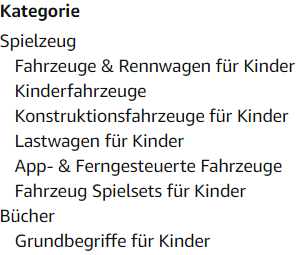
\includegraphics[width=.3\linewidth]{chapters/3_Konzeption/res/Facets/amazon_facet_search_string.png}
    }
    \subfloat[Facettentyp Number]{
        \label{fig:FacetTypes:subfloat:FacetType_Number}
        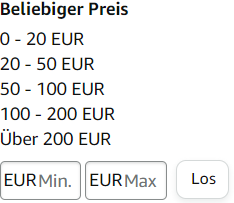
\includegraphics[width=.3\linewidth]{chapters/3_Konzeption/res/Facets/amazon_facet_search_number.png}
    }
    \subfloat[Facettentyp Boolean]{
        \label{fig:FacetTypes:subfloat:FacetType_Boolean}
        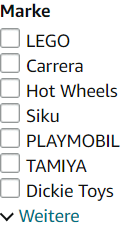
\includegraphics[width=.15\linewidth]{chapters/3_Konzeption/res/Facets/amazon_facet_search_boolean.png}
    }
    \caption{Von Amazon gegebene Facetten, mit eingegebenem Begriff ''Fahrzeug''}
    \label{fig:FacetTypes:Amazon_FacetTypes}
\end{figure}

Die in Abbildung \ref{fig:FacetTypes:Amazon_FacetTypes} gezeigten Facettentypen werden über Amazon bereitgestellt.
Diese sind aufteilbar in Zeichenketten (\ref{fig:FacetTypes:subfloat:FacetType_String}), Zahlen (\ref{fig:FacetTypes:subfloat:FacetType_Number}) und Booleans (\ref{fig:FacetTypes:subfloat:FacetType_Boolean}). Diese drei Typen stellen hierbei die primitiven Datentypen dar \cite{TODO primitivie Datentypen}, wobei Zahlen in ganze und rationale Zahlen unterschieden werden müssen.

Um diese Datentypen abzudecken, erstellen wir die Facettentypen ''Number'', ''String'' und ''Boolean''.
Hierbei müssen die Werte der Facetten mit ihrem jeweiligen Typen übereinstimmen. Das bedeutet, dass Zahlen als Facet\-ten\-wert zum ''Number''-Facetten\-typ gehören, eine Zeichen\-kette als Facetten\-wert zum ''String''-Facetten\-typ usw.
Zeichenketten können jedoch als Datum formatiert werden \cite{TODO Datums-Formatierung}, wodurch sie einen speziellen Typ annehmen können.
Aufgrund dessen sollte auch eine Facette des Types Datum verwendet werden.

Somit gilt:
\begin{description}
    \item[Number Facette:]
    Ein Facettenwert \(v_f\) in der Number Facette \(F_N\) ist eine Zahl oder kann mehrere Zahlen enthalten.
    \\Es gilt: \(\forall v_f \in F_N: v_f \in \mathbb{Q}\)
    \item[Boolean Facette:]
    Ein Facettenwert \(v_f\) in der Boolean Facette \(F_B\) ist entweder ein oder mehrere true oder false Werte.
    \\Es gilt: \(\forall v_f \in F_B: v_f \in \{true, false\}\)
    \item[String Facette:]
    Ein Facettenwert \(v_f\) in der String Facette \(F_S\) ist entweder ein oder mehrere Zeichenketten.
    \\Es gilt: \(\forall v_f \in F_S: v_f \in Alphabet\)
    \item[Date Facette:]
    Ein Facettenwert \(v_f\) in der Date Facette \(F_D\) ist ein Datum.
    \\Es gilt: \(\forall v_f \in F_D: v_f = DATUM\)
\end{description}

%%%%%%%%%%%%%%%%%%%%%%%%%%%%%%%%%%%%%%%%%%%%%%%%%%%%%%%%%%%%%%%%%%%%%%%%%%
\section{Facettenwert-Filterung}
\label{sec:Konzeption:FacetValue_filtering}
Facetten müssen zusätzlich zur Typisierung auch eine Filterung derer Werte aufweisen.
So sieht man beispielsweise in Abbildung \ref{fig:FacetTypes:subfloat:FacetType_Number} eine Bereichseingabe des Preises mit Minimum und Maximum.

Eine String-Facette, zu sehen in Abbildung \ref{fig:FacetTypes:subfloat:FacetType_String}, stellt ledigilich ein Label dar.
Man kann sie jedoch auch so gestalten, dass sie als Suchfunktion dargestellt werden kann. Somit können Nutzer Artikel oder Dokumente nach ihrer jeweiligen Facetten-Suchanfrage filtern.
Beispielsweise könnte man dann, anstelle die Kategorie anzuklicken, die jeweilige Kategorie eintippen.

Facetten des Typs Boolean können hingegen nur zwei mögliche Werte annehmen: Ausgewählt oder nicht ausgewählt, zu sehen in Abbildung \ref{fig:FacetTypes:subfloat:FacetType_Boolean}.

Facetten des Typs Datum können ein oder zwei verschiedene Daten annehmen.
Wird ein spezifisches Datum gewählt, so filtert man die Werte nach diesem einen spezifischen Datum,
werden hingegen zwei verschiedene Werte gewählt, so filtert man nach einem Bereich, der sich durch die zwei Daten ergibt.

Wird keine Facette ausgewählt, so werden alle Artikel/Dokumente angezeigt.

%%%%%%%%%%%%%%%%%%%%%%%%%%%%%%%%%%%%%%%%%%%%%%%%%%%%%%%%%%%%%%%%%%%%%%%%%%
\section{Facetten-IDs}
\label{sec:Konzeption:FacetIDs}
Facetten benötigen eine eindeutige Identifikation, damit diese nicht mehrmals generiert werden.
Semi-strukturierte Daten könnten eine eindeutige Zuweisung in einem extra Feld liefern. 
Da jedoch dynamisch erzeugte Facetten generiert werden und die semi-strukturierten Daten zufällig eingelesen und keinem bestimmten Schema folgen, können sie keine eindeutige Zuweisung liefern.
Jedoch können die jeweiligen Namen der Felder, innerhalb der Daten verwendet werden um einen einmaligen Identifikator zu erzeugen.

\begin{figure}[h]
    \myfloatalign
    \subfloat[JSON mit einem simplen Objekt]{
        \label{fig:facetIds:subfloat:jsonSingleObject}
        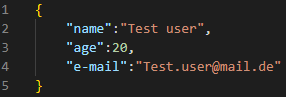
\includegraphics[width=.45\linewidth]{chapters/3_Konzeption/res/Facets/facetgeneration_json_singleObject.png}
    }\quad
    \subfloat[JSON mit einem verschachtelten Objekt]{
        \label{fig:facetIds:subfloat:jsonSingleNestedObject}
        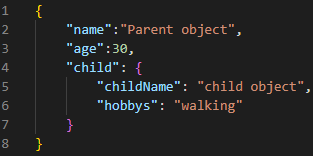
\includegraphics[width=.45\textwidth]{chapters/3_Konzeption/res/Facets/facetgeneration_json_singleObjectNested.png}
    }
    \caption{Darstellung zweier JSON-Objekte.}
    \label{fig:facetIds:jsonObjects}
\end{figure}

Die in Abbildung \ref{fig:facetIds:jsonObjects} gezeigten JSON-Dateien dienen als Darstellungsbeispiel.
Hierbei hat Abbildung \ref{fig:facetIds:subfloat:jsonSingleObject} die Felder: ''name'', ''age'' und ''e-mail'', aus denen die gleichnamigen Facetten generiert werden sollen.

Komplizierter wird es bei dem in Abbildung \ref{fig:facetIds:subfloat:jsonSingleNestedObject} gezeigten verschachtelten JSON-Objekt.
Hierbei gibt es das Feld ''child''. 
Dieses Feld enthält ein weiteres Objekt, mit weiteren Feldern, welche auch zur ID-Generierung in Betracht gezogen werden müssen. 
So sollen ''childName'' und ''hobbys'' auch als Facetten betrachtet werden.
Die IDs sollten hierbei eine Konkatination der Eltern-Facette und der Kind-Facette sein. Das Trennzeichen kann hierbei frei bestimmt werden.
So wären die folgenden IDs das Ergebnis aus der eben genannten Konkatination: ''child.childName'' und ''child.hobbys''.

Damit Nutzer spezifizierter eine Suche angehen können, werden die verschachtelten Facetten nicht zu bereits bestehenden Facetten, wie z.B. ''name'' und ''childName'' hinzugefügt, sondern separat betrachtet.
\input{chapters/3_Konzeption/Parsing}
\section{Architektur}
\label{sec:Konzeption:Architecture}

\begin{figure}[h]
    \centering
    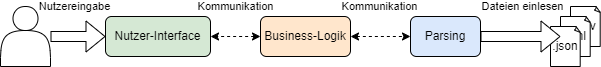
\includegraphics[width=\textwidth]{chapters/3_Konzeption/res/Architektur/class-diagramm_total.png}
    \caption{UML-Klassendiagramm der Anwendung}
    \label{fig:Konzeption:Architektur:UML-Klassendiagramm}
\end{figure}

Die Architektur der Anwendung, zu sehen in Abbildung \ref{fig:Konzeption:Architektur:UML-Klassendiagramm}, soll sich in zwei verschiedene Hauptkomponenten aufteilen, die miteinander kommunizieren: Die Business-Logik, welche sich mit dem Einlesen von Dateien und der dadurch entstehenden Generierung der Facetten auseinandersetzt und dem
Nutzer-Interface, welches die Eingabe des Nutzers annimmt, verarbeitet und an die Business-Logik weitergibt.

    \subsection{Nutzer-Interface}
    \label{subsec:Konzeption:Architektur:UI}

    \begin{figure}[th]
        \centering
        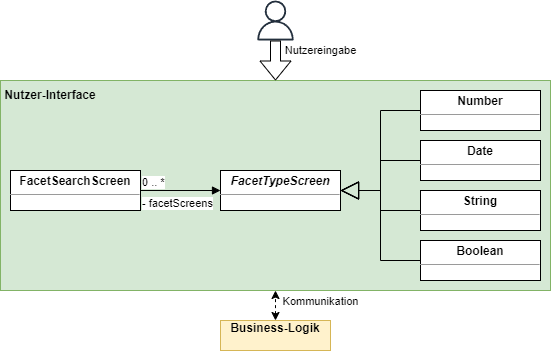
\includegraphics[width=.8\textwidth]{chapters/3_Konzeption/res/Architektur/class-diagramm_User-Interface.png}
        \caption{UML-Klassendagramm des Nutzer-Interfaces}
        \label{fig:Konzeption:Architektur:UI:UML-Klassendiagramm}
    \end{figure}

    Das in Abbildung \ref{fig:Konzeption:Architektur:UI:UML-Klassendiagramm} gezeigte Klassendiagramm stellt jeweils benötigten Komponenten für das User Interface dar, sowie deren Beziehung.

    Man sieht dass die Nutzereingabe über den ''FacetSearchScreen'' erfolgen soll.
    Er besteht aus einem oder mehreren FacetTypeScreens, welche sich auf die jeweiligen Facettentypen, besprochen in \ref{sec:Konzeption:FacetTypes}, zurückführen lassen.
    So repräsentieren NumberScreens die NumberFacetten, DateScreens die DateFacetten, StringScreens die StringFacetten und BooleanScreens die BooleanFacetten.
    Es macht aus Sich des Software Engineerings Sinn, diese Screens aufzuteilen, sodass eine bessere Übersicht, sowie Modularität herrscht.
    Falls man weitere bestimmte Screens hinzufügen oder andere entfernen möchte, so kann man das mithilfe der Vererbung sehr leicht tun.

    Um die jeweiligen Screens für deren entsprechenden Facette auswählen zu können, müssen jedoch zunächst die Facetten generiert werden, dessen Typ man prüfen kann.
    Hierzu wird die Kommunikation zwischen der Business-Logik und dem Nutzer-Interface benötigt.

    \subsection{Business-Logik}
    \label{subsec:Konzeption:Architektur:Business-Logik}

    \begin{figure}[th]
        \centering
        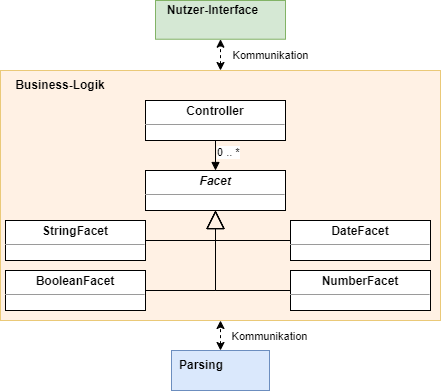
\includegraphics[width=.8\textwidth]{chapters/3_Konzeption/res/Architektur/class-diagramm_Business-Logik.png}
        \caption{UML-Klassendiagramm der Business-Logik}
        \label{fig:Konzeption:Architektur:Business-Logik:UML-Klassendiagramm}
    \end{figure}

    Das in Abbildung \ref{fig:Konzeption:Architektur:Business-Logik:UML-Klassendiagramm} gezeigte Klassendiagramm stellt die jeweiligen Komponenten für die gewollte Business-Logik dar, sowie deren Beziehungen zueinander.

    Hierbei werden die in \ref{sec:Konzeption:FacetTypes} gezeigten Facettentypen übernommen, welche alle von einer Grund-Facette erben sollen.
    Das liegt daran, dass viele Facetten die gleichen Eigenschaften übernehmen können, wie beispielsweise eine Nutzereingabe.
    Jedoch muss, wie in \ref{sec:Konzeption:FacetValue_filtering} erwähnt, auch Funktionen für jeden Facettentyp speziell geliefert werden, wodurch diese einzeln bestimmt werden müssen.

    Des Weiteren erkennt man in Abbildung \ref{fig:Konzeption:Architektur:Business-Logik:UML-Klassendiagramm} auch den Parser, welcher für das Einlesen von Dateien zuständig ist.
    Dieser Parser soll die eingelesenen Dateien dann in eine einheitliche Klasse transformieren, hier ''Document'' genannt.

    Der Controller ist dann für die Generierung der Facetten, sowie weitere logische Schritte notwendig.
    Hierfür benötigt er die ''Document''-Klasse, sodass er anhand der Objekte eben jene Facetten generieren kann.

    \subsection{Parsing}
    \label{subsec:Konzeption:Architektur:Parsing}
    
    \begin{figure}[h]
        \centering
        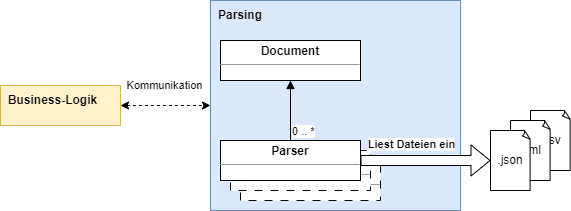
\includegraphics[width=\textwidth]{chapters/3_Konzeption/res/Architektur/class-diagramm_Parsing.png}
        \caption{UML-Klassendiagramm für das Parsing verschiedener Datenformate}
        \label{fig:Konzeption:Architektur:Parsing:Klassendiagramm}
    \end{figure}
    
    In Abbildung \ref{fig:Konzeption:Architektur:Parsing:Klassendiagramm} sind unterschiedliche Parser zu sehen, die ihren jeweiligen Datei-Typen in eine eigene Klasse transformieren.
    Diese Dokumenten-Klasse soll zur Generalisierung der verschiedenen Datenstrukturen verwendet werden, wodurch eine Modularität erzeugt wird, die es zulässt verschiedene Parser für ihre jeweiligen Datei-Strukturen zu entwickeln.
    Hierbei sollen die Dokumente gelesen, verarbeitet und als Dokumenten-Objekte abgespeichert werden.
    Die Business-Logik soll dann auf diese Objekte zugreifen, um aus ihnen die Facetten zu generieren.
    
    So soll es beispielsweise einen JSON-Parser für ''.json''-Dokumente, einen XML-Parser für ''.xml''-Dokumente usw. geben, die diese Dokumenten-Typen dann in ein Dokumenten-Objekt transformieren, mit dem gearbeitet werden kann.
    Die dadurch erzeugte Modularität lässt ein einfaches Hinzufügen oder Entfernen verschiedener Dokumentenstrukturen zu.
\chapter{Implementierung}
\label{ch:Implementierung}
%\chapter{Ein weiteres Kapitel}
\label{ch:chapter03}
liquam facilisis convallis nibh. Ut accumsan malesuada nisi, eget luctus ante dignissim at. Integer dignissim rutrum feugiat. Mauris sit amet leo id ligula fringilla pharetra. In id neque metus, eu congue libero. Suspendisse egestas imperdiet nulla, in blandit dolor venenatis vel. Quisque quis justo quis quam lobortis blandit. Quisque urna mauris, placerat a pretium eu, placerat vel risus. Donec sollicitudin malesuada cursus. Sed auctor aliquet urna sit amet porta. Cum sociis natoque penatibus et magnis dis parturient montes, nascetur ridiculus mus. 

%
% Section: Listen
%
\section{Listen}
\label{sec:chapter03:listen}
Fusce ac velit arcu, in iaculis urna. Vivamus id nunc nulla, et ornare eros. Mauris convallis tortor eget quam interdum nec adipiscing dui pulvinar. Cras a dolor nunc. Sed tincidunt pharetra consectetur. Sed tortor tortor, pellentesque vitae mattis eu, condimentum vel justo.

\begin{itemize}
 \item Enumeration with bullets
 \item Cras cursus ligula et tellus viverra sit amet accumsan orci consequat. Mauris eget elit enim, in mollis justo. Mauris ornare condimentum varius. Praesent suscipit sagittis eros, at accumsan justo adipiscing vel.
 \item Etiam a orci tellus. Cum sociis natoque penatibus et magnis dis parturient montes, nascetur ridiculus mus. Nullam iaculis congue ligula eget lacinia. Proin dapibus elit eu odio egestas dapibus. Etiam nunc dolor, sagittis et volutpat quis, rhoncus a tortor.
\end{itemize}

Nunc non tortor nisl, sed fringilla est. Sed feugiat, est sed imperdiet aliquam, nisl elit lobortis nisl, sit amet ultrices metus eros vitae metus. Integer tincidunt, nisi id consectetur pharetra, nibh tortor tempus ipsum, id sollicitudin erat lacus at diam. Etiam aliquet venenatis aliquet.

\begin{enumerate}
 \item Enumeration with small numbers
 \item Nulla dapibus, ante ac sagittis molestie, neque nulla venenatis turpis, non scelerisque lorem sapien non turpis. Sed dolor magna, vestibulum imperdiet condimentum vel, imperdiet ac mi. Cras in orci egestas purus rhoncus congue. Cras cursus leo nec turpis laoreet non malesuada est pretium.
 \item Nunc ut tortor massa. Fusce ullamcorper mauris eget tellus egestas faucibus. Ut nec nunc quis lectus iaculis ultrices. Lorem ipsum dolor sit amet, consectetur adipiscing elit.
\end{enumerate}

Suspendisse dignissim tellus vitae ante ullamcorper luctus. Maecenas consectetur massa a massa vestibulum non egestas ipsum bibendum. Vestibulum porttitor, tortor at porttitor tristique, magna justo vestibulum sapien, a semper augue magna in orci. Mauris pretium laoreet nisi, sit amet ultricies sapien rutrum ut. Suspendisse placerat risus et magna accumsan. Ased fringilla est. Sed feugiat, est sed imperdiet aliquam, nisl elit lobortis nisl, sit amet ultrices metus eros vitae metus. Integer tincidunt, nisi id consectetur pharetra, nibh tortor tempus ipsum, id sollicitudin erat lacus at diam. Etiam aliquet venenatis aliquet. Mauris sit amet leo id ligula fringilla pharetra. In id neque metus, eu congue libero. Suspendisse egestas imperdiet nulla, in blandit dolor venenatis vel.

\begin{aenumerate}
 \item Enumeration with small caps (alpha)
 \item Second item ed ac risus dolor, ac molestie tellus. Fusce nulla lacus, viverra vel tempus et, viverra eget augue. Nunc id dui sed velit feugiat tristique. Integer at velit justo, eget ornare nulla.
 \item Suspendisse cursus, nisl non pharetra dapibus, nunc ligula sollicitudin sem, in vehicula leo nunc et neque. Sed lacinia dapibus erat, eu dictum ligula auctor a. Phasellus ut mi sapien, in sodales turpis. Nunc pharetra varius metus eget convallis.
\end{aenumerate}

Sia ma sine svedese americas. Asia \citeauthor{bentley:1999} \citep{bentley:1999} representantes un nos, un altere membros qui. De web nostre historia angloromanic. Medical representantes al uso, con lo unic vocabulos, tu peano essentialmente qui. Lo malo laborava anteriormente uso.

\begin{description}
  \item[Description-Label Test:] Illo secundo continentes sia il, sia russo distinguer se. Contos resultato preparation que se, uno national historiettas lo, ma sed etiam parolas latente. Ma unic quales sia. Pan in patre altere summario, le pro latino resultato.
  \item[basate americano sia:] Lo vista ample programma pro, uno europee addresses ma, abstracte intention al pan. Nos duce infra publicava le. Es que historia encyclopedia, sed terra celos avantiate in. Su pro effortio appellate, o.
  \item[Cras venenatis:] Purus et posuere lacinia, nisl sapien dapibus metus, a ornare enim odio in ipsum. Quisque imperdiet nibh metus, in fringilla tellus. Duis varius dui eget orci commodo ac sollicitudin est placerat. Cras varius tincidunt arcu, quis imperdiet nibh rhoncus vel. Sed non justo orci, non accumsan felis. Maecenas condimentum convallis.
\end{description}

%
% Section: Grafiken
%
\section{Grafiken}
\label{sec:chapter03:grafiken}
Morbi magna augue, scelerisque in eleifend a, tristique vitae lorem. Vivamus non elementum nisi. Aliquam erat volutpat. Nunc pharetra, tortor ut adipiscing bibendum, orci ipsum mollis felis, ut euismod eros purus at tellus. Sed blandit eros at ante mattis in elementum tortor pharetra. Vivamus molestie mattis orci. Quisque ullamcorper, purus sit amet luctus viverra, turpis arcu imperdiet eros, sit amet viverra nisi ligula ut felis.

\subsection{Einfache Grafiken}
\label{sec:chapter03:grafiken:simple}
Vestibulum ante ipsum primis in faucibus orci luctus et ultrices posuere cubilia Curae; Donec sed ante odio. Integer semper, nibh id sollicitudin adipiscing, odio elit blandit mi, sit amet luctus mauris velit nec velit. Aenean commodo cursus magna, id mollis sapien gravida eu. Aenean eleifend, leo dignissim sodales mattis, tellus ante tempor nunc, vulputate tristique nisl metus sit amet tellus. Nullam sollicitudin, metus sit amet sagittis interdum, metus purus dapibus lacus, pharetra lobortis erat enim a leo. Suspendisse a augue in purus tempor blandit. Aliquam malesuada porttitor nibh vel adipiscing. In mi est, vulputate nec dapibus quis, pharetra vel lacus. Sed pellentesque egestas pretium. Praesent orci risus, ornare non accumsan id, gravida sed lectus. Mauris fermentum viverra neque at dignissim. Sed consectetur auctor lorem, eget volutpat urna sodales id. Etiam pellentesque velit quis sapien tempus convallis. 

\begin{figure}[htbp]
 \centering
 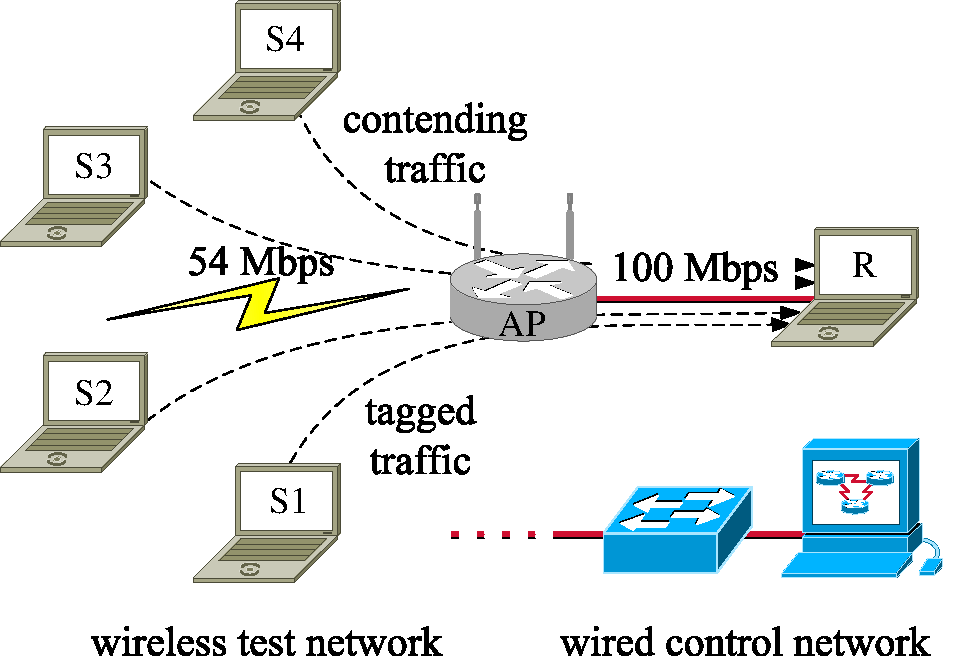
\includegraphics[width=0.5\textwidth]{gfx/examples/setup}
 \caption{Dies ist eine einfache Grafik}
 \label{fig:chapter03:setup}
\end{figure}

Aenean blandit neque eget nunc euismod ac dignissim enim euismod. Nullam semper, orci vitae elementum pretium, est lorem sodales justo, id lobortis nunc felis et justo. Cras tortor orci, rhoncus a commodo quis, aliquam eu dui. Donec pulvinar, arcu ornare consequat ultricies, purus dui accumsan massa, id auctor magna justo nec risus. Nulla bibendum, est nec ornare venenatis, lacus diam pretium augue, sed convallis orci sapien vitae lectus. In blandit massa aliquam felis feugiat fringilla.

\subsection{Grafiken mit Subfloat}
\label{sec:chapter03:grafiken:subfloat}
Quisque non massa neque. In at placerat lacus. Integer urna augue, laoreet ac mattis sed, posuere ut turpis. Nunc a metus quis elit placerat ultricies vel a eros. Quisque condimentum aliquet fermentum. Integer arcu est, suscipit quis lacinia at, volutpat nec tortor. Proin feugiat tristique est eget luctus. Suspendisse porta mauris sed sapien egestas sit amet volutpat tellus ultricies. Nulla vulputate semper turpis sed blandit. Phasellus at tortor pulvinar nisi luctus gravida.

\begin{figure}[bth]
  \myfloatalign
  \subfloat[Asia personas duo.]{
     \label{fig:chapter03:subfloat:grafik1}
     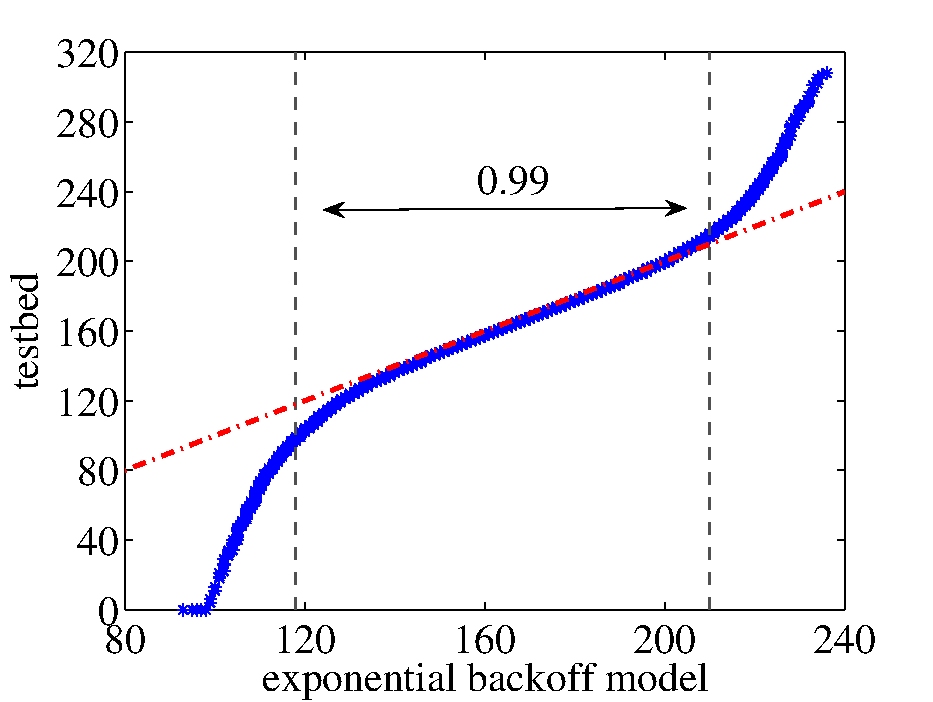
\includegraphics[width=.45\linewidth]{gfx/examples/qq-plot_gaus_vs_160}
   } \quad
   \subfloat[Pan ma signo.] {
     \label{fig:chapter03:subfloat:grafik2}
     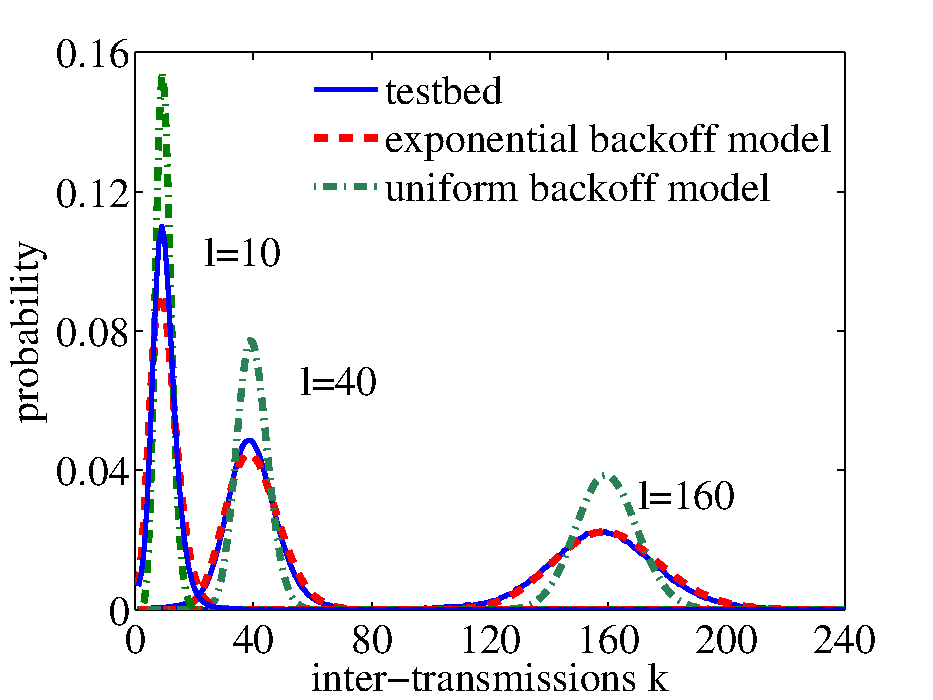
\includegraphics[width=.45\linewidth]{gfx/examples/pdf_gaus_vs_uni_vs_10_40_160}
   } \\
   \subfloat[Methodicamente o uno.]{
     \label{fig:chapter03:subfloat:grafik3}
     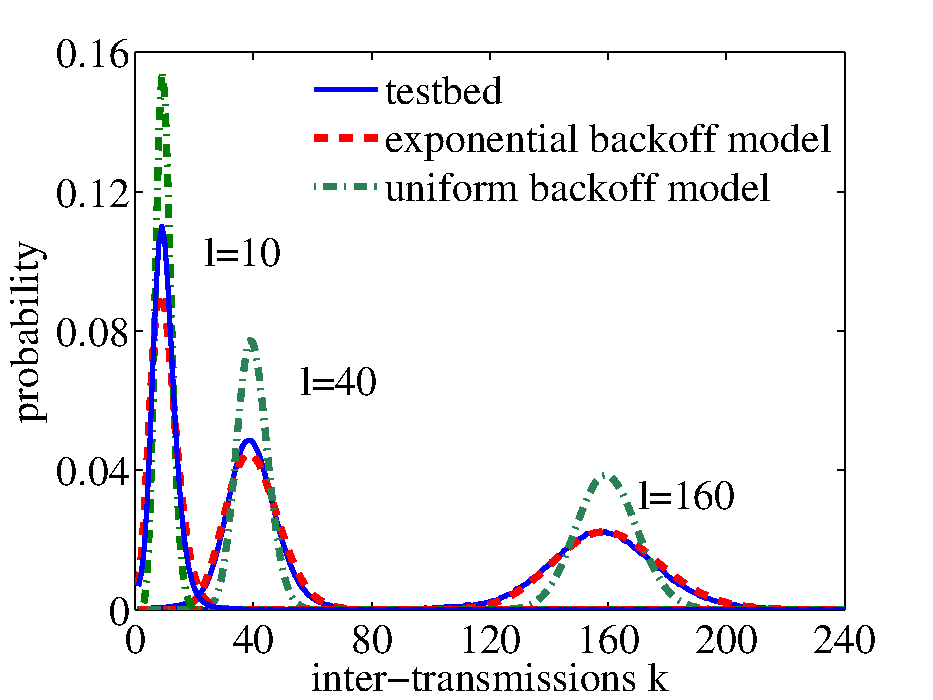
\includegraphics[width=.45\linewidth]{gfx/examples/pdf_gaus_vs_uni_vs_10_40_160}
   } \quad
   \subfloat[Titulo debitas.]{
     \label{fig:chapter03:subfloat:grafik4}
     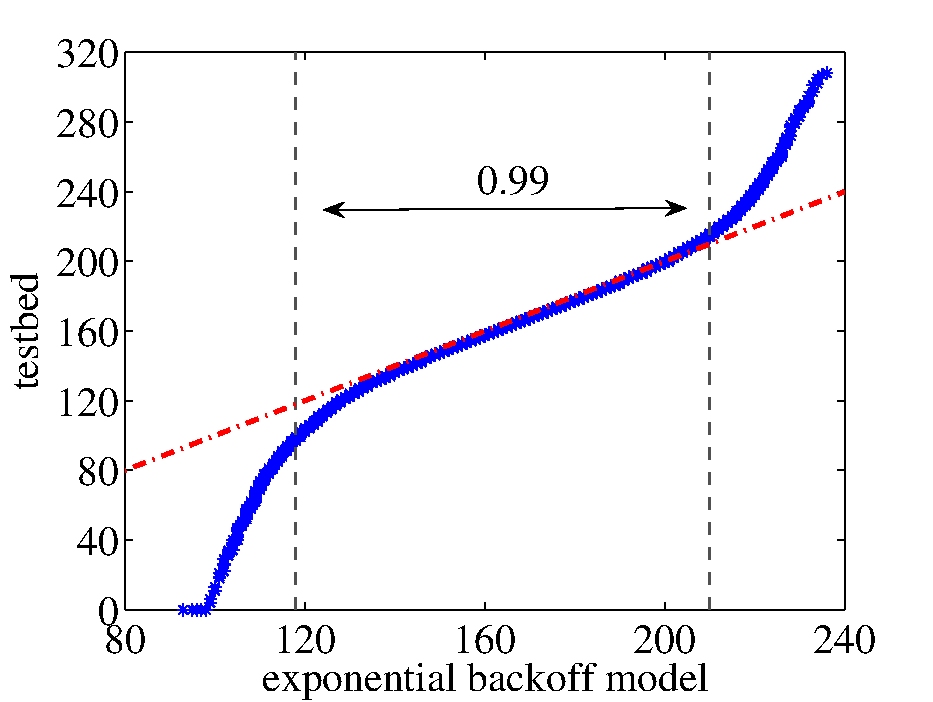
\includegraphics[width=.45\linewidth]{gfx/examples/qq-plot_gaus_vs_160}
   }
   \caption[Subfloat - Figure]{Mit Subfloat lassen sich mehrere Grafiken neben- und untereinander darstellen. Jeder Figure kann dabei mit einem eigenen Text versehen werden.}
   \label{fig:chapter03:subfloat}
\end{figure}


\subsection{Grafiken mit Minipage}
\label{sec:chapter03:grafiken:minipage}
Donec gravida consequat arcu, et mollis tortor posuere vitae. Sed pharetra turpis a ante commodo accumsan. Suspendisse leo nulla, accumsan sit amet dapibus in, posuere eget turpis. Vivamus enim sapien, porta id placerat eget, laoreet sed massa. Class aptent taciti sociosqu ad litora torquent per conubia nostra, per inceptos himenaeos.

\begin{figure}[htbp]
  \centering
  \begin{minipage}[b]{5 cm}
    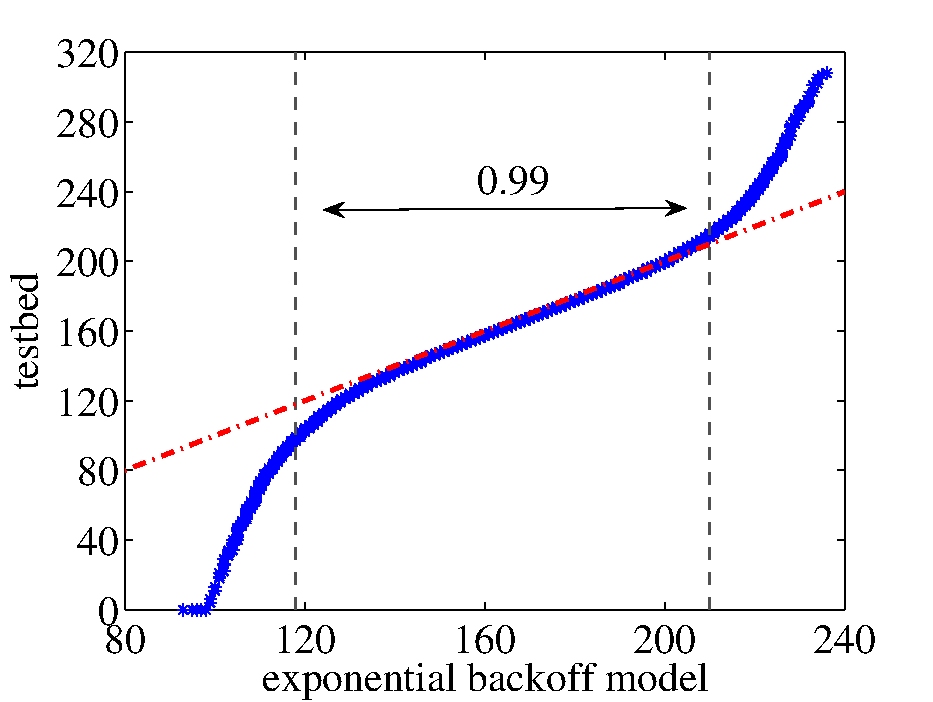
\includegraphics[width=\linewidth]{gfx/examples/qq-plot_gaus_vs_160} 
    \caption{Minipage-Grafik Nummero uno}
    \label{fig:chapter03:minipage:grafik1}
  \end{minipage}
  \begin{minipage}[b]{5 cm}
    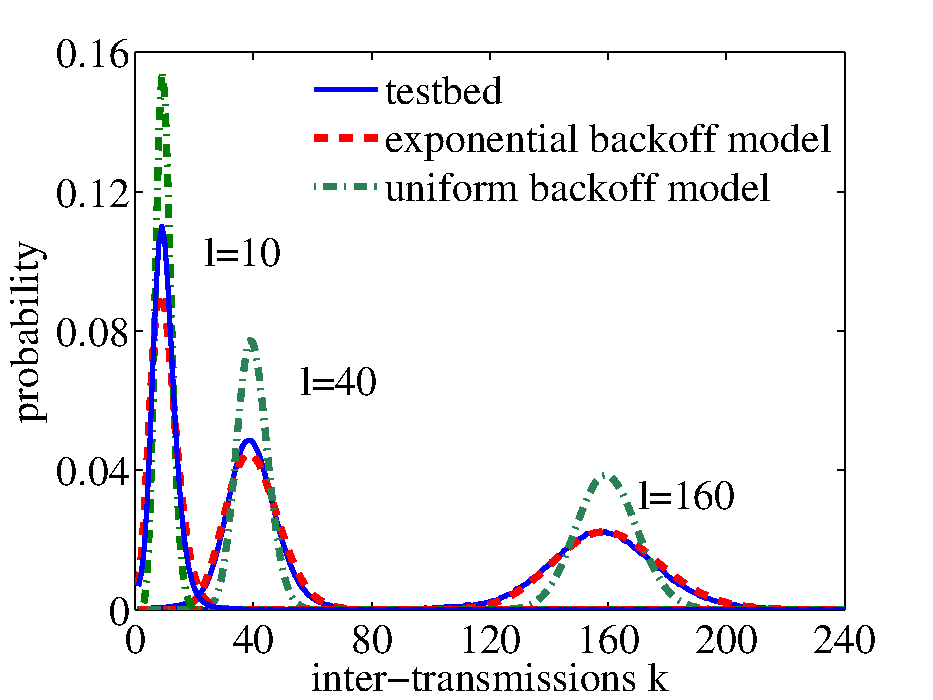
\includegraphics[width=\linewidth]{gfx/examples/pdf_gaus_vs_uni_vs_10_40_160}  
    \caption{Minipage-Grafik Nummer zwei}
    \label{fig:chapter03:minipage:grafik2}
  \end{minipage}
\end{figure}

In vitae est eget velit mattis lobortis. In hac habitasse platea dictumst. Quisque aliquam quam et justo pellentesque ullamcorper. Curabitur elementum mattis leo facilisis tincidunt. Fusce posuere viverra ultricies. Cras eget velit et ipsum gravida imperdiet et hendrerit orci.

Maecenas fringilla viverra urna ut egestas. Nulla sagittis molestie libero eget luctus. Nulla non odio sit amet magna vehicula tincidunt. Nulla accumsan ornare placerat. In posuere scelerisque quam, sed posuere urna eleifend quis. Pellentesque sed quam quis dui vulputate convallis ut ac diam. In hac habitasse platea dictumst. Donec molestie auctor dapibus. Vivamus in erat risus, ut aliquet diam. Duis vel velit ante, id ullamcorper turpis. Lorem ipsum dolor sit amet, consectetur adipiscing elit. In accumsan ornare tellus a porttitor. Etiam facilisis dui et sem eleifend id luctus nisl scelerisque. Aenean quis commodo libero. Nulla quis semper dolor. 

%
% Section: Tabellen 
%
\section{Tabellen}
\label{sec:chapter03:tabellen}
Sed lobortis vestibulum euismod. Vivamus vestibulum gravida nisi vitae condimentum. Nullam nec lacus nibh. Phasellus arcu magna, varius eget viverra a, elementum eu dolor. Aliquam erat volutpat. Sed nibh leo, vestibulum quis lacinia in, vestibulum sollicitudin nulla. In iaculis, purus in imperdiet sagittis, tortor diam pellentesque lectus, eget faucibus ante elit at tortor.

%
% Section: Listings 
%
\section{Listings}
\label{sec:chapter03:listings}
Aliquam ut pretium lectus. Curabitur in eros et sapien aliquet luctus ut sit amet eros. Proin et libero non mi venenatis aliquet at sed lorem. Ut sed enim mi, id viverra eros. Cras metus ante, placerat id commodo at, molestie non libero. Aenean eu risus erat, vel consequat metus. Sed malesuada metus sit amet nisl viverra hendrerit.


%
% Section: Equations
%
\section{Equations}
\label{sec:chapter03:equations}
Pellentesque sed quam quis dui vulputate convallis ut ac diam. In hac habitasse platea dictumst. Donec molestie auctor dapibus. Vivamus in erat risus, ut aliquet diam. Duis vel velit ante, id ullamcorper turpis.
%
\begin{equation}
 U = R * I
\end{equation}

Lorem ipsum dolor sit amet, consectetur adipiscing elit. In accumsan ornare tellus a porttitor. Etiam facilisis dui et sem eleifend id luctus nisl scelerisque. Aenean quis commodo libero. Nulla quis semper dolor.
%
\begin{equation}
 I = \frac{U}{R} 
\end{equation}

In the following we use probability theory to derive closed-form expressions for the fairness that is achieved among $M$ contending stations. We tag station $M$ and denote $K_i$ the inter-transmissions of station $i = 1 \dots M-1$ and let $K = \sum_{i=1}^{M-1} K_i$. The conditional probability $P[K\!=\!k|l]$ can be defined for $M \ge 2$ as
%
\begin{equation}
\mathsf{P}[K\!=\!k|l] = \mathsf{P} \Biggl[\sum_{i=1}^{M-1} K_i = k \Big| l \Biggr]
\label{eq:chapter03:exactpmf}
\end{equation}
%
where the random variables $K_i$ are the integers that satisfy
%
\begin{equation*}
\sum_{j=1}^{K_i} b_i(j) \le \sum_{j=1}^{l} b_M(j) \;\;\; \textmd{and} \;\;\; \sum_{j=1}^{K_i+1} b_i(j) > \sum_{j=1}^{l} b_M(j) .
\end{equation*}


%
% Section: Theorem and Proof
%
\section{Theorem and Proof}
\label{sec:chapter03:theorem}
We use the central limit theorem to derive the long-term fairness. In the sequel, we denote normal random variables $N(\mu,\sigma^2)$ where $\mu$ is the mean and $\sigma^2$ the variance.
%
\begin{Theorem}[Gaussian approximation]
\label{th:chapter03:twostationsgaussian}
%
Let the $b_i(j)$ be i.i.d. random variables with mean $\mu$ and variance $\sigma^2$ and let $M=2$. For $k,l \gg 1$ (\ref{eq:chapter03:exactpmf}) is approximately Gaussian where
%
\begin{equation*}
\mathsf{P}[K \!\le\! k|l] \approx \mathsf{P}\biggl[ N(0,1) \le \frac{\mu\,(k-l)}{\sigma\,\sqrt{k+l}} \biggr] .
\end{equation*}
%
\end{Theorem}
%
\begin{proof}
%
For $M=2$ we have from (\ref{eq:chapter03:exactpmf}) that
%
\begin{equation*}
\mathsf{P}[K \!<\! k|l] = \mathsf{P} \Biggl[\, \sum_{j=1}^k b_1(j) > \sum_{j=1}^l b_2(j) \Biggr]
\end{equation*}
%
and after expansion and some normalization this equals
%
\begin{equation*}
= \mathsf{P}\Biggl[ \frac{\sum_{j=1}^{l}b_2(j) - l\mu}{\sigma\sqrt{l}} - \frac{\sum_{j=1}^{k}b_1(j) - k\mu}{\sigma\sqrt{l}} < \frac{\mu(k-l)}{\sigma\sqrt{l}} \Biggr].
\end{equation*}
%
Using the central limit theorem it follows that
%
\begin{equation*}
\mathsf{P}[K \!<\! k|l] \approx \mathsf{P} \biggl[ N(0,1) - N \biggl(0,\frac{k}{l}\biggr) < \frac{\mu(k-l)}{\sigma\sqrt{l}} \biggr] .
\end{equation*}
%
Since the normal distribution with zero mean is symmetric we can replace the subtraction of $N(0,k/l)$ by addition. Furthermore, the sum of two normal random variables $N(\mu_1, \sigma_1^2)$ and $N(\mu_2, \sigma_2^2)$ is normal with $N(\mu_1+\mu_2, \sigma_1^2+ \sigma_2^2)$ such that
%
\begin{equation*}
\mathsf{P}[K \!<\! k|l] \approx \mathsf{P} \biggl[ N\biggl(0,\frac{k+l}{l}\biggr) < \frac{\mu(k-l)}{\sigma\sqrt{l}} \biggr] .
\end{equation*}
%
Finally, we use that if $X$ is $N(a\mu,a^2\sigma^2)$ then $Y = X/a$ is $N(\mu,\sigma^2)$ with $a^2 = (k+l)/l$ to standardize the result.
%
\end{proof}

Th. \ref{th:chapter03:twostationsgaussian} assumes i.i.d. random countdown values. It does, however, not make any assumption about their distribution.

%*************************************************************************
% Recommendations
%*************************************************************************
%\part{Empfehlungen zur Erstellung wissenschaftlicher Abschlussarbeiten}
%\label{pt:recommendations}
%*************************************************************************
% Backmatter
%*************************************************************************
\appendix
%\renewcommand{\thechapter}{\alph{chapter}}
\cleardoublepage
\part{Appendix}
%************************************************
\chapter{Introduction to the ClassicThesis style}\label{ch:classicthesis}
%************************************************
The ClassicThesis bundle for \LaTeX\ has two goals:
\begin{enumerate}
    \item Provide students with an easy-to-use template for their
    Master's
    or PhD thesis. (Though it might also be used by other types of
    authors
    for reports, books, etc.)
    \item Provide a classic, high-quality typographic style that is
    inspired by \citeauthor{bringhurst:2002}'s ``\emph{The Elements of
    Typographic Style}'' \citep{bringhurst:2002}.
    \marginpar{\myTitle \myVersion}
\end{enumerate}
The bundle is configured to run with a \emph{full}
MiK\TeX\ or \TeX Live\footnote{See the file \texttt{LISTOFFILES} for
needed packages. Furthermore, \texttt{classicthesis}
works with most other distributions and, thus, with most systems
\LaTeX\ is available for.}
installation right away and, therefore, it uses only freely available
fonts. (Minion fans can easily adjust the style to their needs.)

People interested only in the nice style and not the whole bundle can
now use the style stand-alone via the file \texttt{classicthesis.sty}.
This works now also with ``plain'' \LaTeX.

As of version 3.0, \texttt{classicthesis} can also be easily used with
\mLyX\footnote{\url{http://www.lyx.org}} thanks to Nicholas Mariette
and Ivo Pletikosić. The \mLyX\ version of this manual will contain
more information on the details.

This should enable anyone with a basic knowledge of \LaTeXe\ or \mLyX\ to
produce beautiful documents without too much effort. In the end, this
is my overall goal: more beautiful documents, especially theses, as I
am tired of seeing so many ugly ones.

The whole template and the used style is released under the
\acsfont{GNU} General Public License.

If you like the style then I would appreciate a postcard:
\begin{center}
    André Miede \\
    Detmolder Straße 32 \\
    31737 Rinteln \\
    Germany
\end{center}
The postcards I received so far are available at:
\begin{center}
    \url{http://postcards.miede.de}
\end{center}
\marginpar{A well-balanced line width improves the legibility of
the text. That's what typography is all about, right?}
So far, many theses, some books, and several other publications have
been typeset successfully with it. If you are interested in some
typographic details behind it, enjoy Robert Bringhurst's wonderful book.
% \citep{bringhurst:2002}.

\paragraph{Important Note:} Some things of this style might look
unusual at first glance, many people feel so in the beginning.
However, all things are intentionally designed to be as they are,
especially these:
\begin{itemize}
    \item No bold fonts are used. Italics or spaced small caps do the
    job quite well.
    \item The size of the text body is intentionally shaped like it
    is. It supports both legibility and allows a reasonable amount of
    information to be on a page. And, no: the lines are not too short.
    \item The tables intentionally do not use vertical or double
    rules. See the documentation for the \texttt{booktabs} package for
    a nice discussion of this topic.\footnote{To be found online at
    \url{http://mirror.ctan.org/macros/latex/contrib/booktabs/}.}
    \item And last but not least, to provide the reader with a way
    easier access to page numbers in the table of contents, the page
    numbers are right behind the titles. Yes, they are \emph{not}
    neatly aligned at the right side and they are \emph{not} connected
    with dots that help the eye to bridge a distance that is not
    necessary. If you are still not convinced: is your reader
    interested in the page number or does she want to sum the numbers
    up?
\end{itemize}
Therefore, please do not break the beauty of the style by changing
these things unless you really know what you are doing! Please.

\paragraph{Yet Another Important Note:} Since \texttt{classicthesis}'
first release in 2006, many things have changed in the \LaTeX\ world.
Trying to keep up-to-date, \texttt{classicthesis} grew and evolved
into many directions, trying to stay (some kind of) stable and be
compatible with its port to \mLyX. However, there are still many
remains from older times in the code, many dirty workarounds here and
there, and several other things I am absolutely not proud of (for
example my unwise combination of \acsfont{KOMA} and
\texttt{titlesec} etc.).
\graffito{An outlook into the future of \texttt{classicthesis}.}

Currently, I am looking into how to completely re-design and
re-implement \texttt{classicthesis} making it easier to maintain and
to use. As a general idea, \texttt{classicthesis.sty} should be
developed and distributed separately from the template bundle itself.
Excellent spin-offs such as \texttt{arsclassica} could also be
integrated (with permission by their authors) as format configurations.
Also, current trends of \texttt{microtype}, \texttt{fontspec}, etc.
should be included as well. As I am not really into deep
\LaTeX\ programming,
I will reach out to the \LaTeX\ community for their expertise and help.


\section{Organization}
A very important factor for successful thesis writing is the
organization of the material. This template suggests a structure as
the following:
\begin{itemize}
    \marginpar{You can use these margins for summaries of the text
    body\dots}
    \item\texttt{Chapters/} is where all the ``real'' content goes in
    separate files such as \texttt{Chapter01.tex} etc.
    % \item\texttt{Examples/} is where you store all listings and other
    % examples you want to use for your text.
    \item\texttt{FrontBackMatter/} is where all the stuff goes that
    surrounds the ``real'' content, such as the acknowledgments,
    dedication, etc.
    \item\texttt{gfx/} is where you put all the graphics you use in
    the thesis. Maybe they should be organized into subfolders
    depending on the chapter they are used in, if you have a lot of
    graphics.
    \item\texttt{Bibliography.bib}: the Bib\TeX\ database to organize
    all the references you might want to cite.
    \item\texttt{classicthesis.sty}: the style definition to get this
    awesome look and feel. Does not only work with this thesis template
    but also on its own (see folder \texttt{Examples}). Bonus: works
    with both \LaTeX\ and \textsc{pdf}\LaTeX\dots and \mLyX.
    % \item\texttt{ClassicThesis.tcp} a \TeX nicCenter project file.
    Great tool and it's free!
    \item\texttt{ClassicThesis.tex}: the main file of your thesis
    where all gets bundled together.
    \item\texttt{classicthesis-config.tex}: a central place to load all
    nifty packages that are used. % In there, you can also activate
    % backrefs in order to have information in the bibliography about
    % where a source was cited in the text (\ie, the page number).

    \emph{Make your changes and adjustments here.} This means that you
    specify here the options you want to load \texttt{classicthesis.sty}
    with. You also adjust the title of your thesis, your name, and all
    similar information here. Refer to \autoref{sec:custom} for more
    information.

    This had to change as of version 3.0 in order to enable an easy
    transition from the ``basic'' style to \mLyX.
\end{itemize}
In total, this should get you started in no time.


\clearpage
\section{Style Options}\label{sec:options}
There are a couple of options for \texttt{classicthesis.sty} that
allow for a bit of freedom concerning the layout:
\marginpar{\dots or your supervisor might use the margins for some
    comments of her own while reading.}
\begin{itemize}
    \item General:
        \begin{itemize}
            \item\texttt{drafting}: prints the date and time at the bottom of
            each page, so you always know which version you are dealing with.
            Might come in handy not to give your Prof. that old draft.
        \end{itemize}

    \item Parts and Chapters:
        \begin{itemize}
            \item\texttt{parts}: if you use Part divisions for your document,
            you should choose this option. (Cannot be used together with
            \texttt{nochapters}.)

            \item\texttt{linedheaders}: changes the look of the chapter
            headings a bit by adding a horizontal line above the chapter
            title. The chapter number will also be moved to the top of the
            page, above the chapter title.
        \end{itemize}

    \item Typography:
        \begin{itemize}
            \item\texttt{eulerchapternumbers}: use figures from Hermann Zapf's
            Euler math font for the chapter numbers. By default, old style
            figures from the Palatino font are used.

            \item\texttt{beramono}: loads Bera Mono as typewriter font.
            (Default setting is using the standard CM typewriter font.)

            \item\texttt{eulermath}: loads the awesome Euler fonts for math.
            Pala\-tino is used as default font.
        \end{itemize}

    \marginpar{Options are enabled via \texttt{option=true}}

    \item Table of Contents:
        \begin{itemize}
            \item\texttt{tocaligned}: aligns the whole table of contents on
            the left side. Some people like that, some don't.

            \item\texttt{dottedtoc}: sets pagenumbers flushed right in the
            table of contents.

            \item\texttt{manychapters}: if you need more than nine chapters for
            your document, you might not be happy with the spacing between the
            chapter number and the chapter title in the Table of Contents.
            This option allows for additional space in this context.
            However, it does not look as ``perfect'' if you use
            \verb|\parts| for structuring your document.
        \end{itemize}

    \item Floats:
        \begin{itemize}
            \item\texttt{listings}: loads the \texttt{listings} package (if not
            already done) and configures the List of Listings accordingly.

            \item\texttt{floatperchapter}: activates numbering per chapter for
            all floats such as figures, tables, and listings (if used).
        \end{itemize}

\end{itemize}

Furthermore, pre-defined margins for different paper sizes are available, \eg, \texttt{a4paper}, \texttt{a5paper}, and \texttt{letterpaper}. These are based on your chosen option of \verb|\documentclass|.

The best way to figure these options out is to try the different
possibilities and see what you and your supervisor like best.

In order to make things easier, \texttt{classicthesis-config.tex}
contains some useful commands that might help you.


\section{Customization}\label{sec:custom}
%(As of v3.0, the Classic Thesis Style for \LaTeX{} and \mLyX{} share
%the same two \texttt{.sty} files.)
This section will show you some hints how to adapt
\texttt{classicthesis} to your needs.

The file \texttt{classicthesis.sty}
contains the core functionality of the style and in most cases will
be left intact, whereas the file \texttt{classic\-thesis-config.tex}
is used for some common user customizations.

The first customization you are about to make is to alter the document
title, author name, and other thesis details. In order to do this, replace
the data in the following lines of \texttt{classicthesis-config.tex:}%
\marginpar{Modifications in \texttt{classic\-thesis-config.tex}%
}

\begin{lstlisting}
    % **************************************************
    % 2. Personal data and user ad-hoc commands
    % **************************************************
    \newcommand{\myTitle}{A Classic Thesis Style\xspace}
    \newcommand{\mySubtitle}{An Homage to...\xspace}
\end{lstlisting}

Further customization can be made in \texttt{classicthesis-config.tex}
by choosing the options to \texttt{classicthesis.sty}
(see~\autoref{sec:options}) in a line that looks like this:

\begin{lstlisting}
  \PassOptionsToPackage{
    drafting=true,    % print version information on the bottom of the pages
    tocaligned=false, % the left column of the toc will be aligned (no indentation)
    dottedtoc=false,  % page numbers in ToC flushed right
    parts=true,       % use part division
    eulerchapternumbers=true, % use AMS Euler for chapter font (otherwise Palatino)
    linedheaders=false,       % chaper headers will have line above and beneath
    floatperchapter=true,     % numbering per chapter for all floats (i.e., Figure 1.1)
    listings=true,    % load listings package and setup LoL
    subfig=true,      % setup for preloaded subfig package
    eulermath=false,  % use awesome Euler fonts for mathematical formulae (only with pdfLaTeX)
    beramono=true,    % toggle a nice monospaced font (w/ bold)
    minionpro=false   % setup for minion pro font; use minion pro small caps as well (only with pdfLaTeX)
  }{classicthesis}
\end{lstlisting}

Many other customizations in \texttt{classicthesis-config.tex} are
possible, but you should be careful making changes there, since some
changes could cause errors.

% Finally, changes can be made in the file \texttt{classicthesis.sty},%
% \marginpar{Modifications in \texttt{classicthesis.sty}%
% } although this is mostly not designed for user customization. The
% main change that might be made here is the text-block size, for example,
% to get longer lines of text.


\section{Issues}\label{sec:issues}
This section will list some information about problems using
\texttt{classic\-thesis} in general or using it with other packages.

Beta versions of \texttt{classicthesis} can be found at Bitbucket:
\begin{center}
    \url{https://bitbucket.org/amiede/classicthesis/}
\end{center}
There, you can also post serious bugs and problems you encounter.


\section{Future Work}
So far, this is a quite stable version that served a couple of people
well during their thesis time. However, some things are still not as
they should be. Proper documentation in the standard format is still
missing. In the long run, the style should probably be published
separately, with the template bundle being only an application of the
style. Alas, there is no time for that at the moment\dots it could be
a nice task for a small group of \LaTeX nicians.

Please do not send me email with questions concerning \LaTeX\ or the
template, as I do not have time for an answer. But if you have
comments, suggestions, or improvements for the style or the template
in general, do not hesitate to write them on that postcard of yours.


\section{Beyond a Thesis}
The layout of \texttt{classicthesis.sty} can be easily used without the
framework of this template. A few examples where it was used to typeset
an article, a book or a curriculum vitae can be found in the folder
\texttt{Examples}. The examples have been tested with
\texttt{latex} and \texttt{pdflatex} and are easy to compile. To
encourage you even more, PDFs built from the sources can be found in the
same folder.


\section{License}
\paragraph{GNU General Public License:} This program is free software;
you can redistribute it and/or modify
it under the terms of the \acsfont{GNU} General Public License as
published by
the Free Software Foundation; either version 2 of the License, or
(at your option) any later version.

This program is distributed in the hope that it will be useful,
but \emph{without any warranty}; without even the implied warranty of
\emph{merchant\-ability} or \emph{fitness for a particular purpose}.
See the
\acsfont{GNU} General Public License for more details.

You should have received a copy of the \acsfont{GNU} General
Public License
along with this program; see the file \texttt{COPYING}.  If not,
write to
the Free Software Foundation, Inc., 59 Temple Place - Suite 330,
Boston, MA 02111-1307, USA.

\paragraph{classichthesis Authors' note:} There have been some discussions about the GPL's implications on using \texttt{classicthesis} for theses etc. Details can be found here:
\begin{center}
  \url{https://bitbucket.org/amiede/classicthesis/issues/123/}
\end{center}

We chose (and currently stick with) the GPL because we would not like to compete with proprietary modified versions of our own work. However, the whole template is free as free beer and free speech. We will not demand the sources for theses, books, CVs, etc. that were created using \texttt{classicthesis}.

Postcards are still highly appreciated.





%*****************************************
%*****************************************
%*****************************************
%*****************************************
%*****************************************

%********************************************************************
% Appendix
%*******************************************************
% If problems with the headers: get headings in appendix etc. right
%\markboth{\spacedlowsmallcaps{Appendix}}{\spacedlowsmallcaps{Appendix}}
\chapter{Appendix Test}
Lorem ipsum at nusquam appellantur his, ut eos erant homero
concludaturque. Albucius appellantur deterruisset id eam, vivendum
partiendo dissentiet ei ius. Vis melius facilisis ea, sea id convenire
referrentur, takimata adolescens ex duo. Ei harum argumentum per. Eam
vidit exerci appetere ad, ut vel zzril intellegam interpretaris.
\graffito{More dummy text.}

%Errem omnium ea per, pro congue populo ornatus cu, ex qui dicant
%nemore melius. No pri diam iriure euismod. Graecis eleifend
%appellantur quo id. Id corpora inimicus nam, facer nonummy ne pro,
%kasd repudiandae ei mei. Mea menandri mediocrem dissentiet cu, ex
%nominati imperdiet nec, sea odio duis vocent ei. Tempor everti
%appareat cu ius, ridens audiam an qui, aliquid admodum conceptam ne
%qui. Vis ea melius nostrum, mel alienum euripidis eu.

\section{Appendix Section Test}
Test: \autoref{tab:moreexample} (This reference should have a
lowercase, small caps \spacedlowsmallcaps{A} if the option
\texttt{floatperchapter} is activated, just as in the table itself
 $\rightarrow$ however, this does not work at the moment.)

\begin{table}[h]
    \myfloatalign
    \begin{tabularx}{\textwidth}{Xll} \toprule
        \tableheadline{labitur bonorum pri no} & \tableheadline{que vista}
        & \tableheadline{human} \\ \midrule
        fastidii ea ius & germano &  demonstratea \\
        suscipit instructior & titulo & personas \\
        %postulant quo & westeuropee & sanctificatec \\
        \midrule
        quaestio philosophia & facto & demonstrated \\
        %autem vulputate ex & parola & romanic \\
        %usu mucius iisque & studio & sanctificatef \\
        \bottomrule
    \end{tabularx}
    \caption[Autem usu id]{Autem usu id.}
    \label{tab:moreexample}
\end{table}

%Nulla fastidii ea ius, exerci suscipit instructior te nam, in ullum
%postulant quo. Congue quaestio philosophia his at, sea odio autem
%vulputate ex. Cu usu mucius iisque voluptua. Sit maiorum propriae at,
%ea cum primis intellegat. Hinc cotidieque reprehendunt eu nec. Autem
%timeam deleniti usu id, in nec nibh altera.




\section{Another Appendix Section Test}
Equidem detraxit cu nam, vix eu delenit periculis. Eos ut vero
constituto, no vidit propriae complectitur sea. Diceret nonummy in
has, no qui eligendi recteque consetetur. Mel eu dictas suscipiantur,
et sed placerat oporteat. At ipsum electram mei, ad aeque atomorum
mea. There is also a useless Pascal listing below: \autoref{lst:useless}.

\begin{lstlisting}[float=b,language=Pascal,frame=tb,caption={A floating example (\texttt{listings} manual)},label=lst:useless]
for i:=maxint downto 0 do
begin
{ do nothing }
end;
\end{lstlisting}

%Ei solet nemore consectetuer nam. Ad eam porro impetus, te choro omnes
%evertitur mel. Molestie conclusionemque vel at, no qui omittam
%expetenda efficiendi. Eu quo nobis offendit, verterem scriptorem ne
%vix.


%*************************************************************************
% Other Stuff in the Back
%*************************************************************************
\cleardoublepage%********************************************************************
% Bibliography
%*******************************************************
% work-around to have small caps also here in the headline
% https://tex.stackexchange.com/questions/188126/wrong-header-in-bibliography-classicthesis
% Thanks to Enrico Gregorio
\defbibheading{bibintoc}[\bibname]{%
  \phantomsection
  \manualmark
  \markboth{\spacedlowsmallcaps{#1}}{\spacedlowsmallcaps{#1}}%
  \addtocontents{toc}{\protect\vspace{\beforebibskip}}%
  \addcontentsline{toc}{chapter}{\tocEntry{#1}}%
  \chapter*{#1}%
}

% allow Linebreaks in urls anywhere
\setcounter{biburlnumpenalty}{100}
\setcounter{biburlucpenalty}{100}
\setcounter{biburllcpenalty}{100}
% enable to long words to break anywhere by increasing the allowed whitespace between words.
\sloppy

\printbibliography[heading=bibintoc]

%*************************************************************************
% Game Over: Restore, Restart, or Quit?
%*************************************************************************
\end{document}
%*************************************************************************
